\documentclass[journal]{IEEEtran}
\usepackage{graphicx}
\usepackage{amsmath}
\usepackage{amssymb}
\usepackage{amsxtra}
\usepackage{amstext}
\usepackage{latexsym}
%\usepackage{dsfont}
\usepackage{float}
\usepackage{cite}
\usepackage{epstopdf}
\usepackage{multirow}
\usepackage{subcaption}
\hfuzz=\maxdimen
 \tolerance=10000
 \hbadness=10000
\ifCLASSINFOpdf
%\usepackage[pdftex]{graphicx}
  % declare the path(s) where your graphic files are
  % \graphicspath{{../pdf/}{../jpeg/}}
  % and their extensions so you won't have to specify these with
  % every instance of \includegraphics
  % \DeclareGraphicsExtensions{.pdf,.jpeg,.png}
\else

\fi

\hyphenation{op-tical net-works semi-conduc-tor}


\begin{document}
\title{Polarization performance analysis of linear polarized antenna in 2.45GHz on-body communications}

\author{Lingfeng~Liu,~\IEEEmembership{}
        Xiaonan~Wang,~\IEEEmembership{}
        and~Peng~Zhang.~\IEEEmembership{}
\thanks{Lingfeng liu, Xiaonan Wang and Zhang Peng are with the Signal Information Engineering school, East China Jiaotong
University, China, e-mail: lingf.liu@gmail.com.}% <-this % stops a space
\thanks{This work is supported by the Natural Science Foundation of China (NSFC) under grant No. 81460275.}% <-this % stops a
\thanks{Manuscript submitted July 4, 2017.}}


\maketitle

\begin{abstract}
In this paper, three kinds of compact linearly polarized antennas are proposed, and the effects of horizontal polarization
and vertical polarization on the polarization performance of the antenna are analyzed based on the simulation. Antennas are
inverted F antenna, MIFA and printed dipole. Simulated human chest model includes skin, fat��muscle three-tier structure.
The results show that the change of resonant frequency is small after loading the human body, but the radiation orientation
of the antenna is more obvious due to the coupling effect of the human body, and the bandwidth, center frequency and S11 are
affected by the distance between the antenna and the body surface and the relative orientation. After loading the human
body, the resonant frequency of the antenna changes little, the pattern is relatively stable.
\end{abstract}

% Note that keywords are not normally used for peerreview papers.
\begin{IEEEkeywords}
IFA, MIFA, printed dipole, horizontal polarization, vertical polarization, Body Area Network(BAN).
\end{IEEEkeywords}

\IEEEpeerreviewmaketitle



\section{Introduction}
\IEEEPARstart{R}{cent} years, the use of cellular phones and other personal communication services has gradually widened,
making the focus of research on the human body wearing antennas. In the WBAN communication system, the 2.4GHz frequency band
is widely used in various areas of WBAN, such as health care in the health of the monitoring and prevention of health and the
detection of attitude and motion in fitness in the entertainment due to the small size of the antenna, high transmission rate
and low power consumption. Characteristics of antennas and propagation channels in on-body communications have been
ascertained \cite{1}-\cite{4}. At present, some textile patch antennas had been proposed for wearable applications \cite{5}, most of
the research is placed the antenna in the shape of the phone on the head of the assumptions for simulation and testing
\cite{6, 7}, but the wearing antenna is usually placed in the human body torso or limbs, the recent studies have shown that
these are optimal locations for wearable antennas \cite{8}.

Studies as \cite{9, 10} also reveal the possibility to explore the polarization spatial diversity in on-body channels to
improve the performance of e.g. realying and Multi-Input Multi-Output (MIMO) in WBANs. In the study of the antenna on body
surface, the following problems usually arise: the antenna is integrated in the clothing or placed on the human body surface
\cite{11, 12}. The human body can be seen as a media of complex characteristics and must have an impact on antenna performance
parameters \cite{13, 14}. At the same time the distance between antenna and human body is also one of the important factors.
In order to study the impacts of these factors on antenna performance, three kinds of linear polarized antennas were selected
and placed on the surface of the human body. The antenna performance was observed by changing the distance between antenna and
the human body. This paper consists of five parts, the second part introduces the desgin of three kinds of
linear polarized antennas and the third part introduces human body modeling. The fourth part analyse the polarization performance of the antennas. Finally, the performance of the linear polarization antenna in 2.45GHz body surface communication is summarized.
\section{ANTENNAS DESGIN}
We choose IFA, MIFA and printed dipole three microstrip antennas for the study. They have small size, simple structure, low
production costs and also easy to match. Their structure and initial values are shown in Fig. \ref{fig:1} and Tab. \ref{tab:1}.
These antennas are fabricated on the PCB and operates in the 2.4GHz ISM band with the center frequency of 2.45GHz. The
dielectric layer is made of the most commonly FR4 with $\epsilon_{r}$=4.4\cite{15}. The antenna is simulated by Ansoft HFSS
13.0$^{\textcircled{R}}$. After appropriate analysis and optimization of the values of the main parameters, when
\textit{L}=16.2mm, \textit{H}=3.8mm and \textit{S}=5mm, the resonant frequency of IFA is 2.45GHz, the bandwidth is about
450MHz. While \textit{L1} = 3.5 and \textit{GndX} = 34 mm \cite{16}, the resonant frequency is around 2.45 GHz and the
bandwidth is about 225 MHz. While \textit{L2} = 21mm, \textit{L3}= 6mm, the maximum bandwidth is 550MHz and achieve a good
impedance matching at 2.45GHz.The simulation results of three antennas are shown in Fig. \ref{fig:2}.

\begin{table}[!ht]
\centering
\begin{tabular}{|c|c|c|}
\hline
Antennas&Variable&Initial Values\\
\hline
\multirow{7}{*}{IFA}&L&16.2\\
&H&3.8\\
&S&5\\
&W&1\\
&SubH&0.8\\
&GndX&50\\
&GndY&90\\
\hline
\multirow{8}{*}{Dipole}&H&11.6\\
&W1&3\\
&L1&22\\
&W2&3\\
&L2&21\\
&L3&10\\
&L4&12\\
&W3&3\\
\hline
\multirow{8}{*}{MIFA}&D1&0.5\\
&D2&0.3\\
&D3&0.3\\
&D4&0.5\\
&D5&1.4\\
&D6&1.7\\
&L1&3.3\\
&L2&2.7\\
&L3&5\\
&L4&2.64\\
&L5&2\\
&L6&4.9\\
&W1&0.9\\
&W2&0.5\\
\hline
\end{tabular}
\caption{Variable definition}
\label{tab:1}
\end{table}

\begin{figure}[!htb]
\centering
\begin{subfigure}[b]{0.24\textwidth}
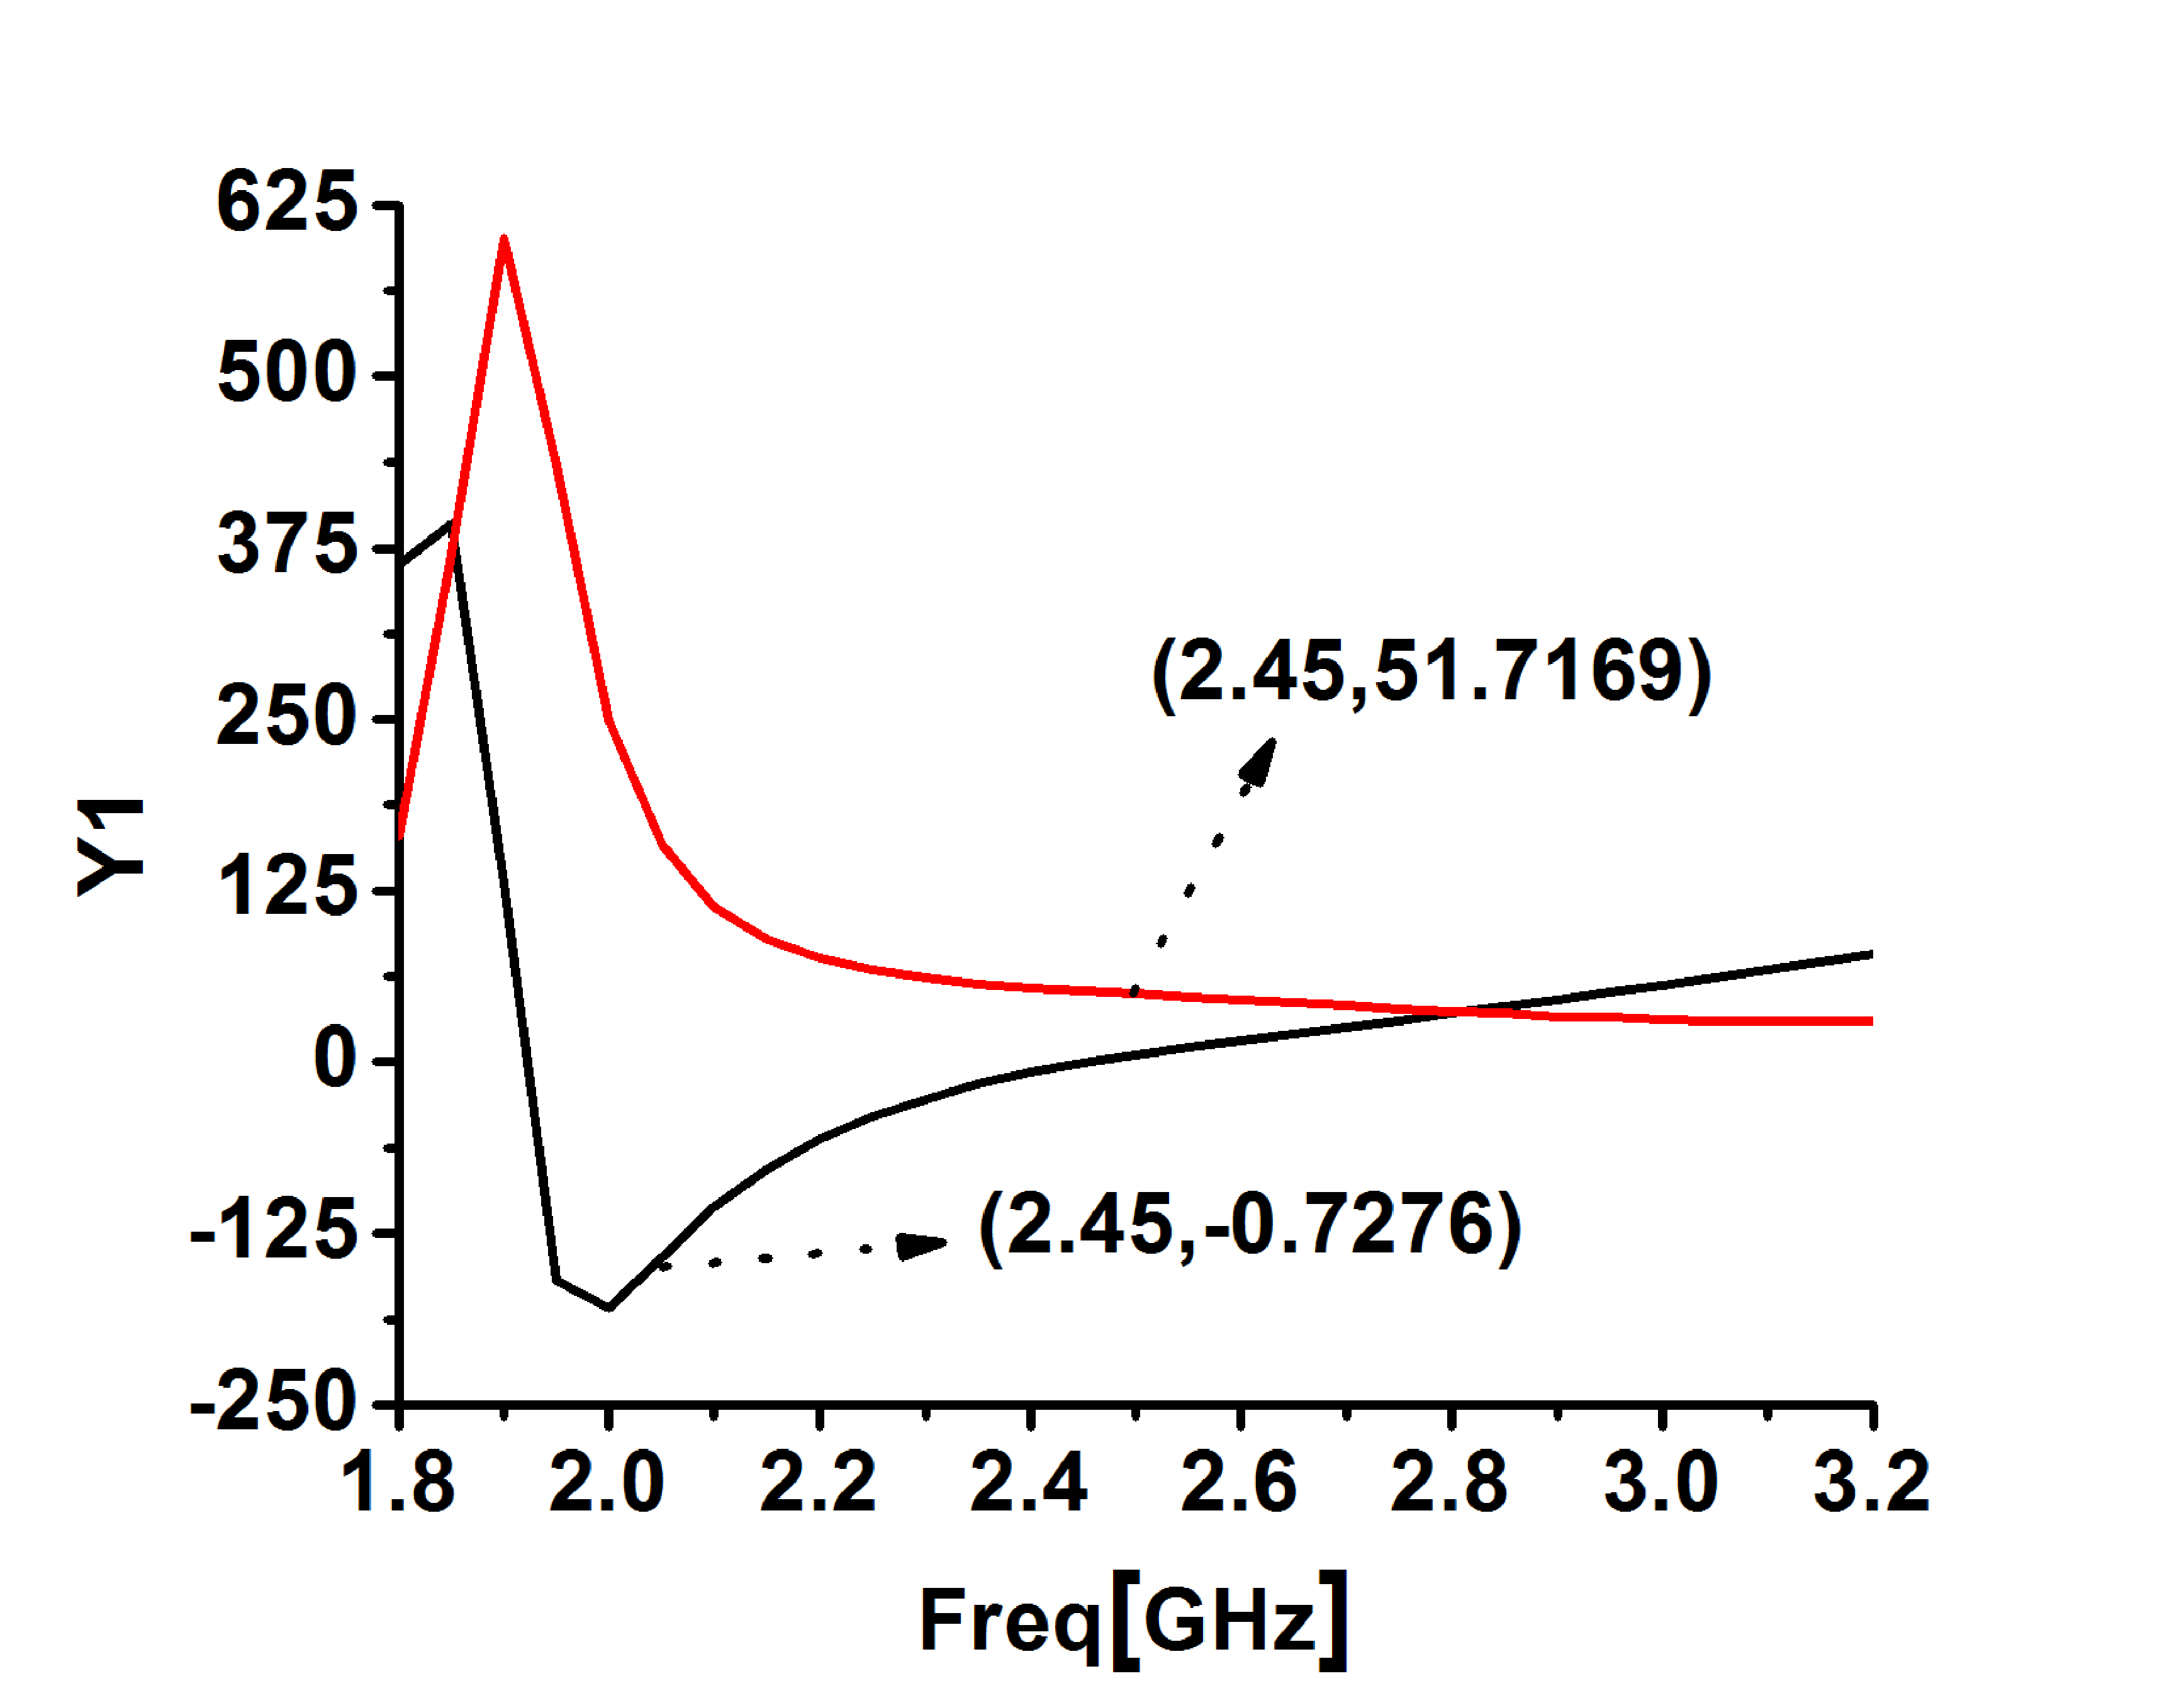
\includegraphics[width=\textwidth]{figs/1c.eps}
\caption{IFA}
\label{fig:a}	
\end{subfigure}		
\begin{subfigure}[b]{0.24\textwidth}
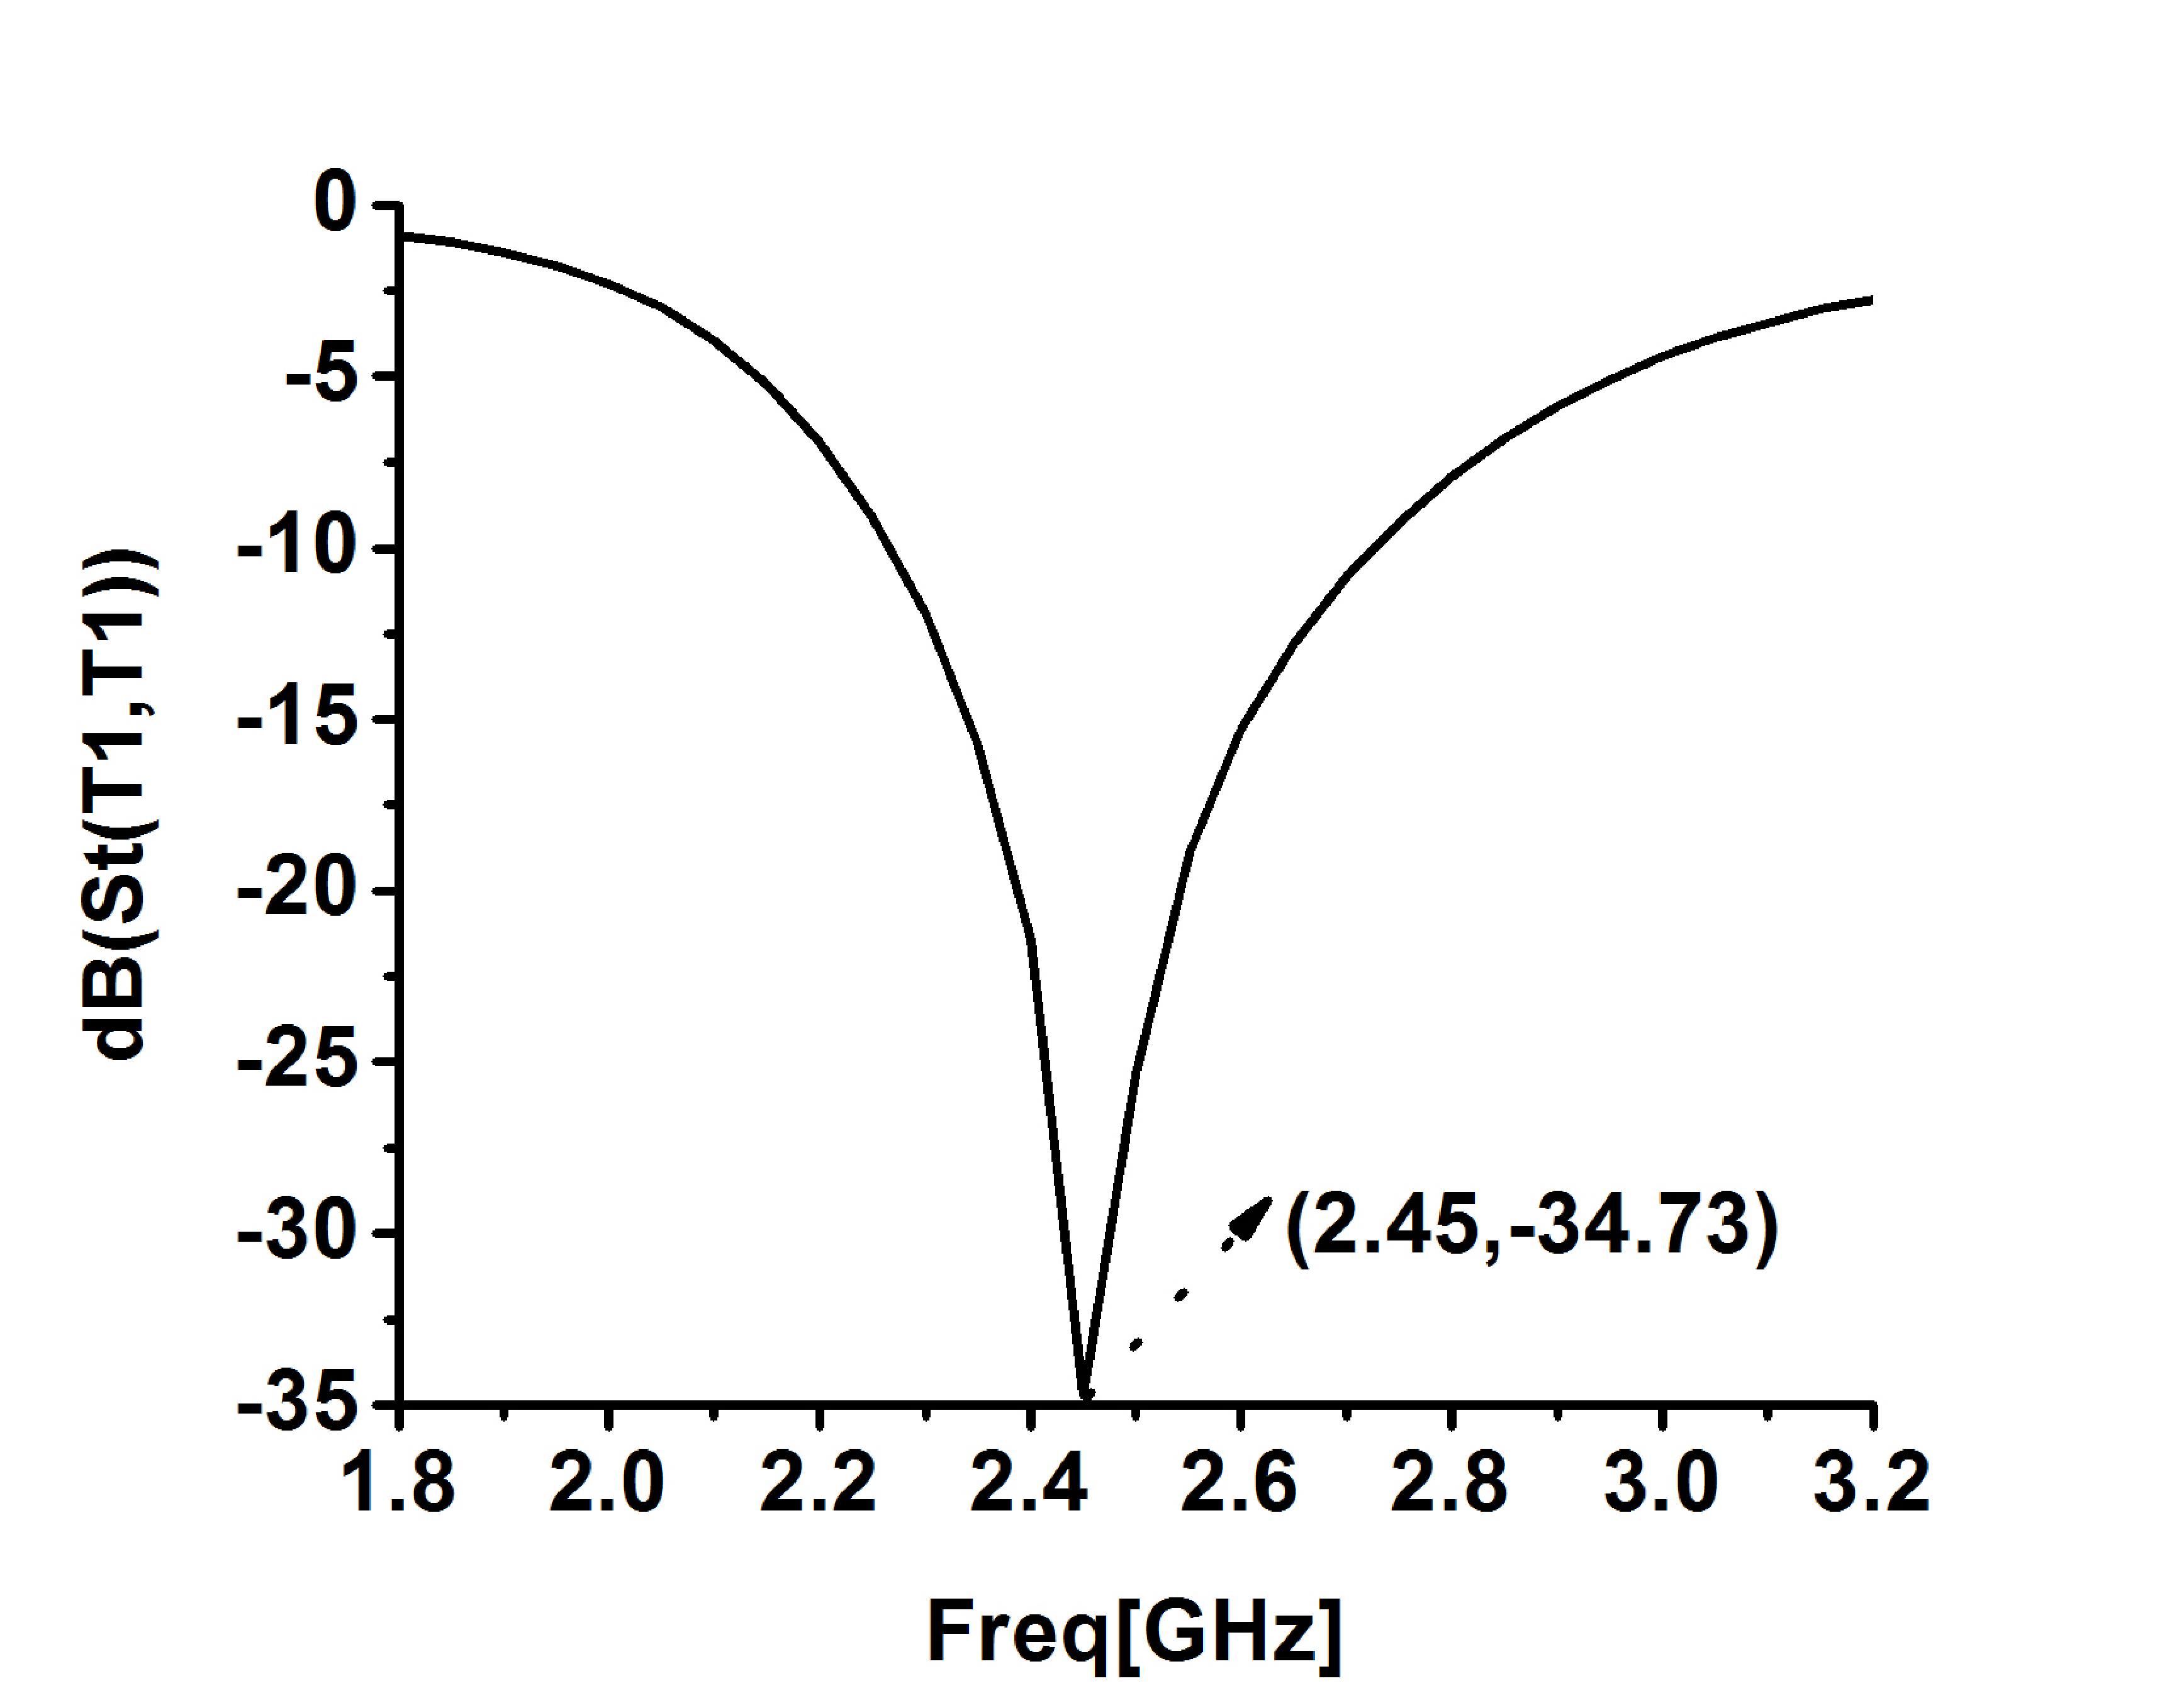
\includegraphics[width=\textwidth]{figs/1b.eps}
\caption{MIFA}
\label{fig:b}
\end{subfigure}
\begin{subfigure}[b]{0.4\textwidth}
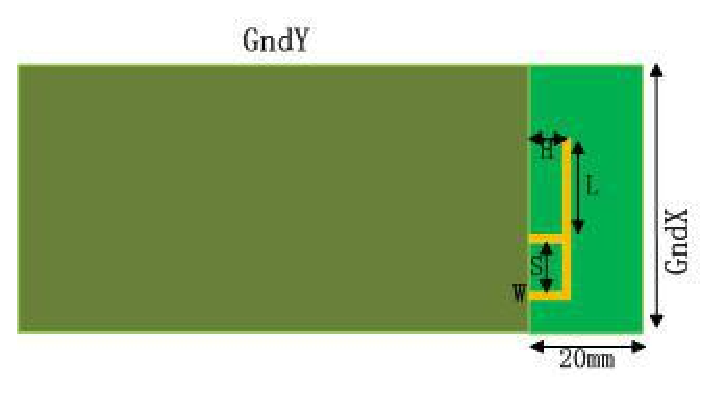
\includegraphics[width=\textwidth]{figs/1a.eps}
\caption{Dipole}
\label{fig:c}
\end{subfigure}
\caption{Parameters of  three antennas}
\label{fig:1}
\end{figure}

\begin{figure}[!htb]
\centering
\begin{subfigure}[b]{0.24\textwidth}
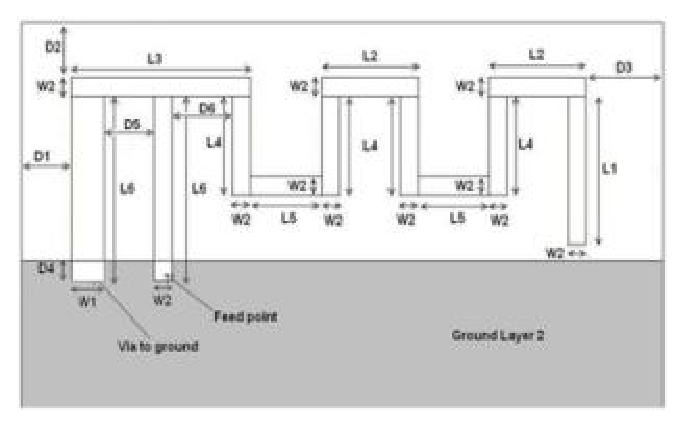
\includegraphics[width=\textwidth]{figs/2a.eps}
\caption{IFA}
\label{fig:2a}	
\end{subfigure}		
\begin{subfigure}[b]{0.24\textwidth}
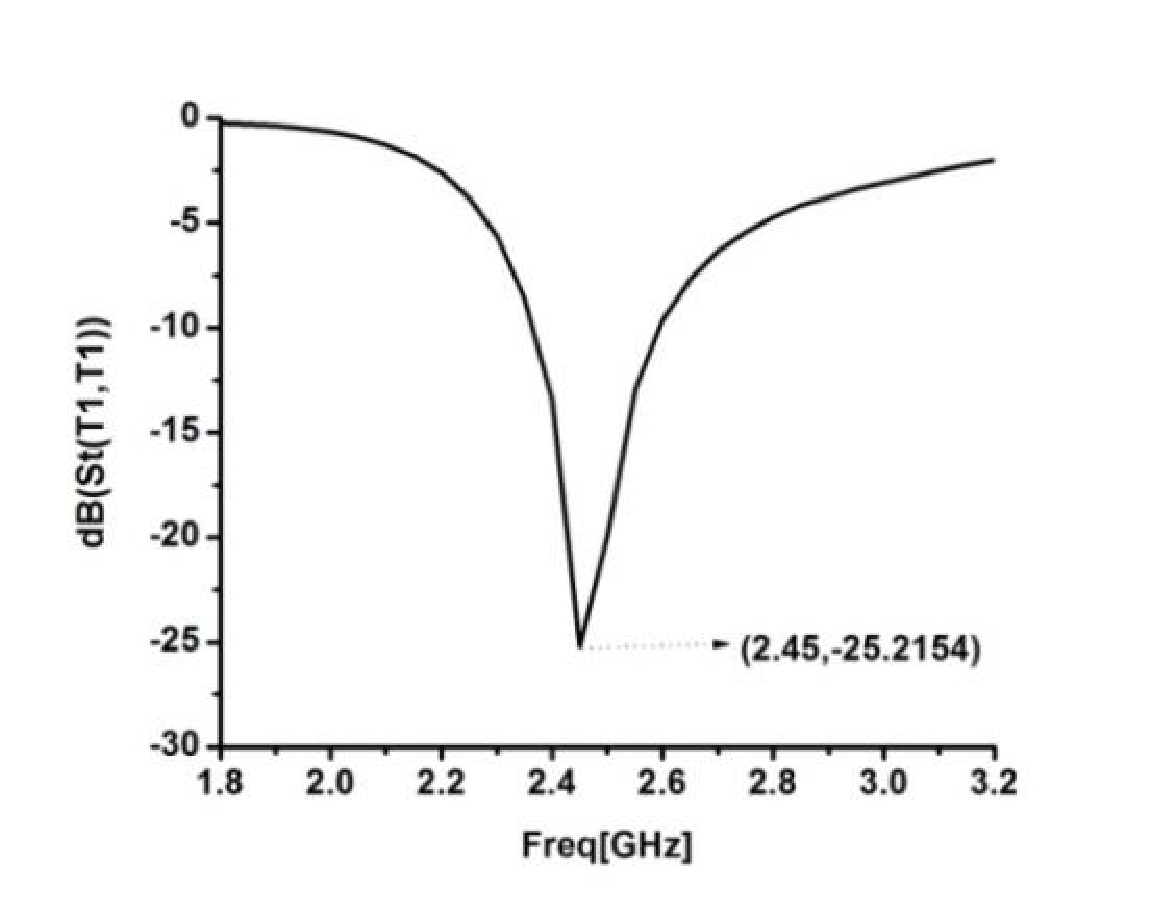
\includegraphics[width=\textwidth]{figs/2b.eps}
\caption{MIFA}
\label{fig:2b}
\end{subfigure}
\begin{subfigure}[b]{0.24\textwidth}
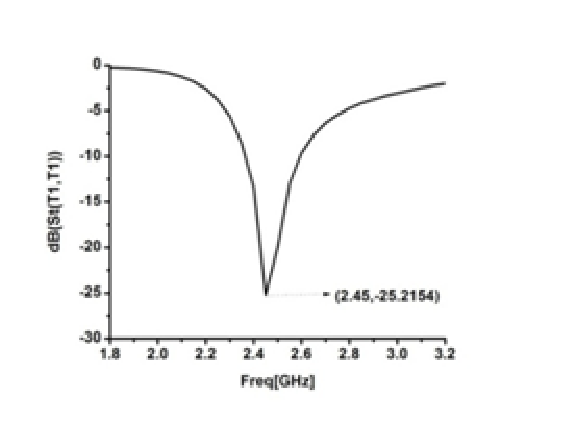
\includegraphics[width=\textwidth]{figs/2c.eps}
\caption{Dipole}
\label{fig:2c}
\end{subfigure}
\caption{Optimized S11}
\label{fig:2}
\end{figure}

\section{HUMAN BODY MODELING}
We must establish the human body model accurately in the study of the impact of human body on antenna, the human body is
composed of various biological tissues with different shapes and electromagnetic properties. Most of the biological tissues
are non-uniform dispersion medium and human body can��t be accurately modeled. We can construct different human models
to obtain multiple results as much as possible within allowable range of the error.
\begin{figure}[!htb]
\centering
\begin{subfigure}[b]{0.24\textwidth}
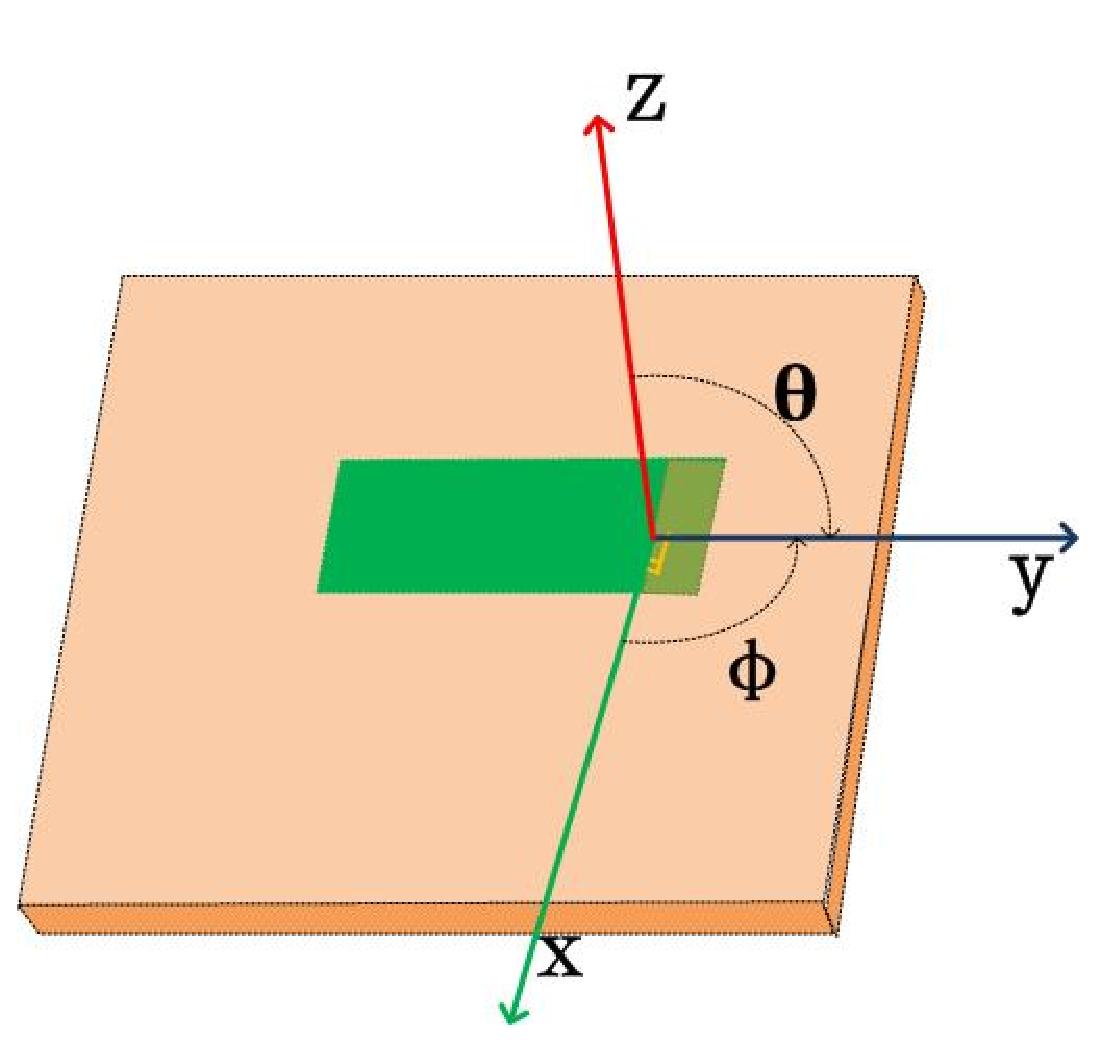
\includegraphics[width=\textwidth]{figs/3a.eps}
\caption{Horizontal polarization}
\label{fig:3a}	
\end{subfigure}		
\begin{subfigure}[b]{0.24\textwidth}
\includegraphics[width=\textwidth]{figs/3b.eps}
\caption{Vertical polarization}
\label{fig:3b}
\end{subfigure}
\begin{subfigure}[b]{0.4\textwidth}
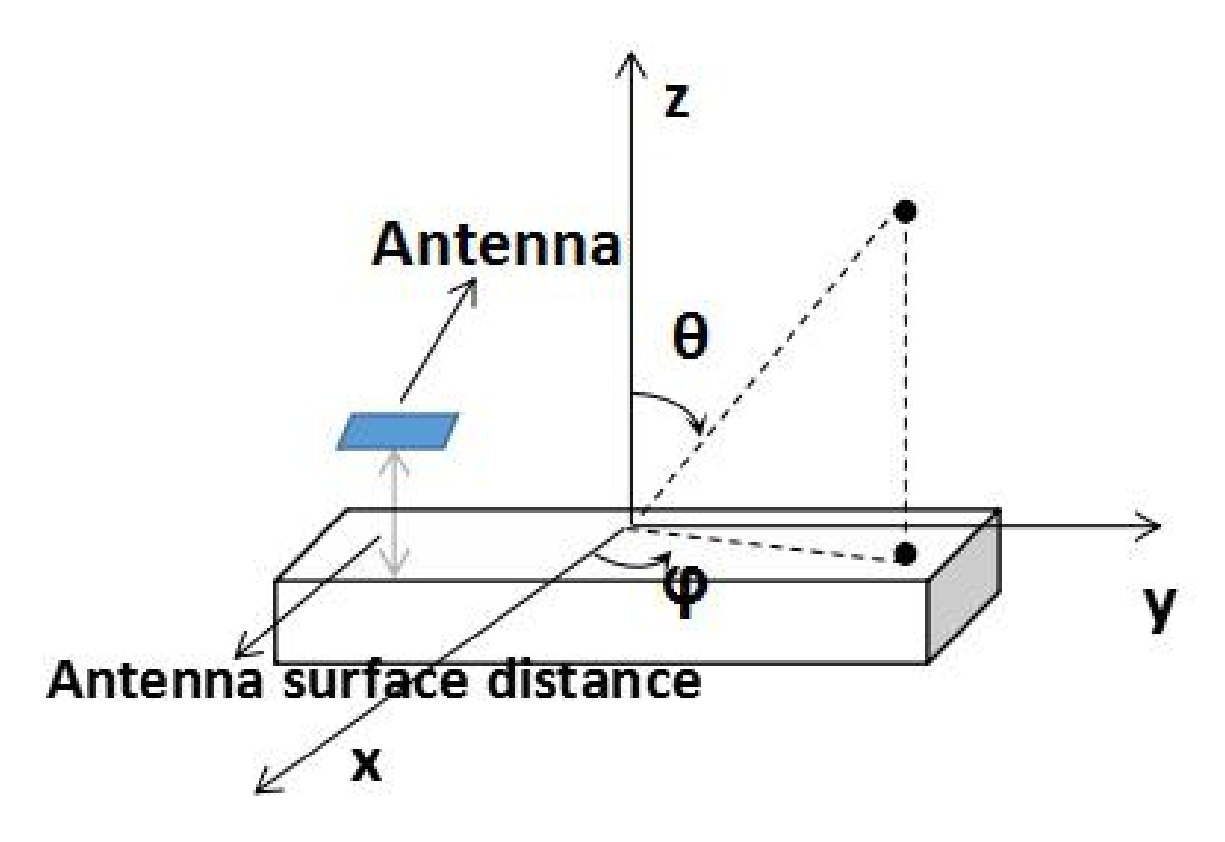
\includegraphics[width=\textwidth]{figs/3c.eps}
\caption{Definition of antenna and body surface distance}
\label{fig:3c}
\end{subfigure}
\caption{Polarization and geometry definition}
\label{fig:3}
\end{figure}
Analysis of antenna performance in realistic environment is subjected to the body shape and environment, we simulate in the
simulation state. As the antenna is not directly in vicinity of the human body, we place a cube simulated human chest at a
certain distance from the antenna as shown in Fig. \ref{fig:3}. The cube is a three layered biological tissue model \cite{17}
. As shown in Fig. \ref{fig:4}, the three-layer structure of the skin layer (2 mm), fat layer (5 mm) and muscle layer (10 mm)
was set from top to the bottom, and the model volume was 200 mm * 160 mm * 17 mm. Considering that the 2.4 GHz signal is
rapidly attenuated in human body, this structure is considered to be able to adequately simulate the human body. Dielectric
constant and other electrical characteristics \cite{17} are derived from human body and shown in Tab. \ref{tab:2}.
\begin{figure}[!htb]
\centering
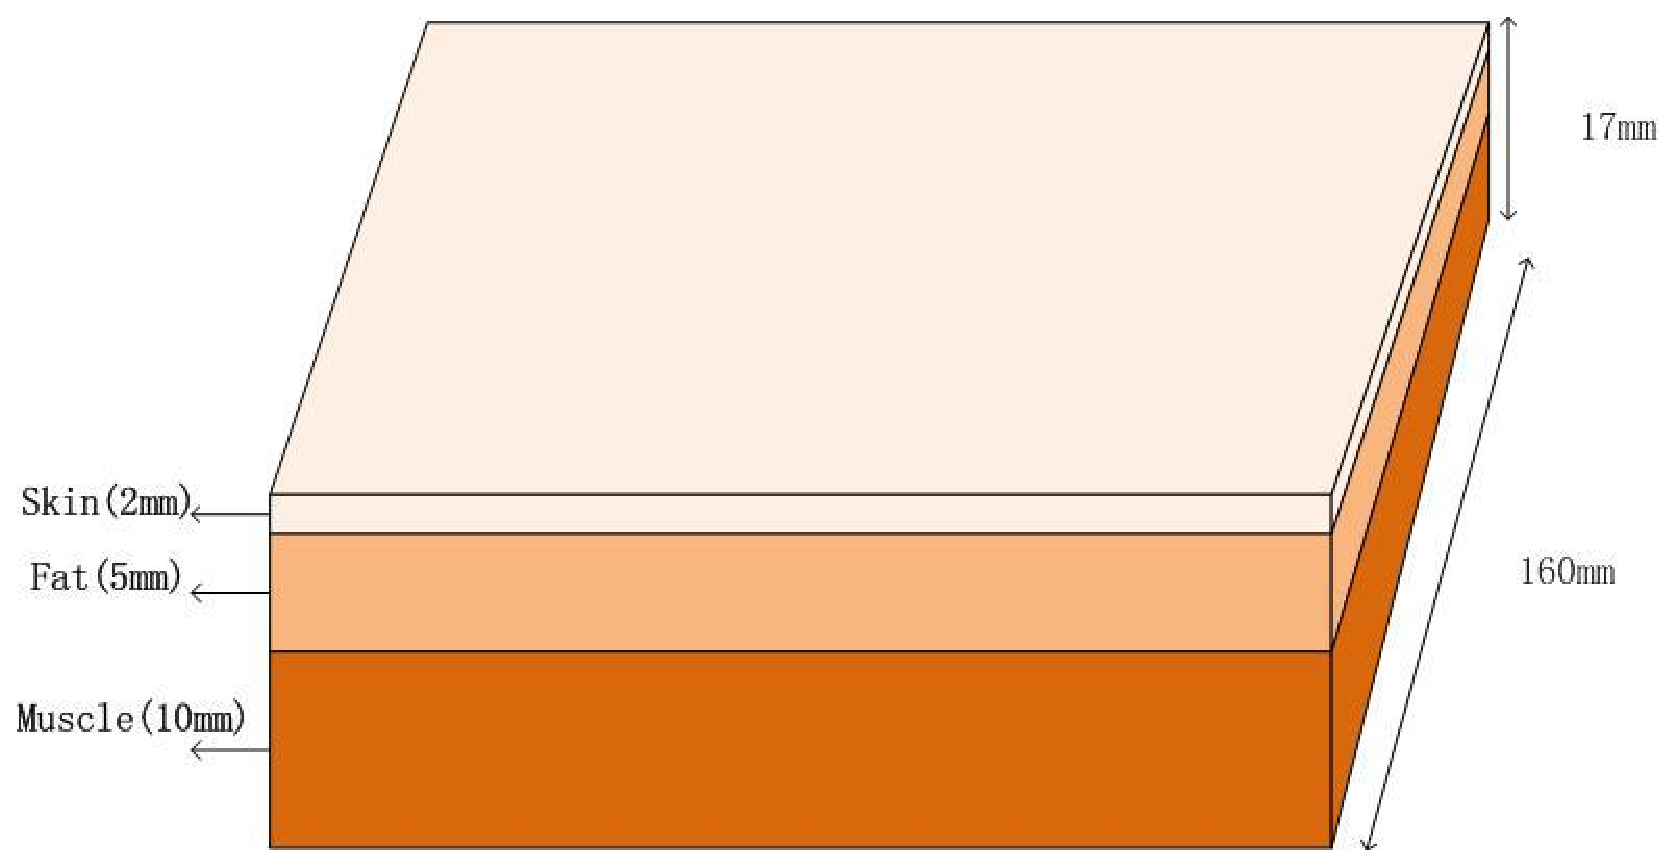
\includegraphics[width=0.4\textwidth]{figs/4.eps}
\caption{Body modeling}
\label{fig:4}	
\end{figure}
\begin{table}[!htb]
\centering
\begin{tabular}{|c|c|c|}
\hline
Tissue&$\epsilon_{r}$&$\sigma$\\
\hline
Skin&38.0066&1.4638\\
\hline
Muscle&52.7295&1.7388\\
Fat&10.8206&0.2680\\
\hline
\end{tabular}
\caption{Chest model parameters at 2.45 GHZ}
\label{tab:2}
\end{table}
\section{Analysis of antenna polarization performance}
The focus of this paper is to observe the antenna performance after loading human by changing the antenna placement. The
distance between the antenna and human body surface(\textit{d}) is an important factor of antenna performance. We summarize
the variation of S11 and bandwidth(\textit{B}) in the range of 0.5cm$<\textit{d}<$6cm , and compare the changes of antenna
gain pattern of different \textit{d}.
\subsection{IFA}
Fig. \ref{fig:5} shows the changes of antenna matching performance and bandwidth of \textit{d}. For horizontal polarization,
0.4GHz\textless\textit{B}\textless0.52GHz, when \textit{d}= 2.5cm, \textit{B} reaches the maximum; for vertical polarization,
the fitting equation for the bandwidth is
\begin{equation}
\label{eq:eps_1}
y[GHz]=0.0628x+0.1845,   x[cm]
\end{equation}
\begin{figure}[!htb]
\centering
\begin{subfigure}[b]{0.4\textwidth}
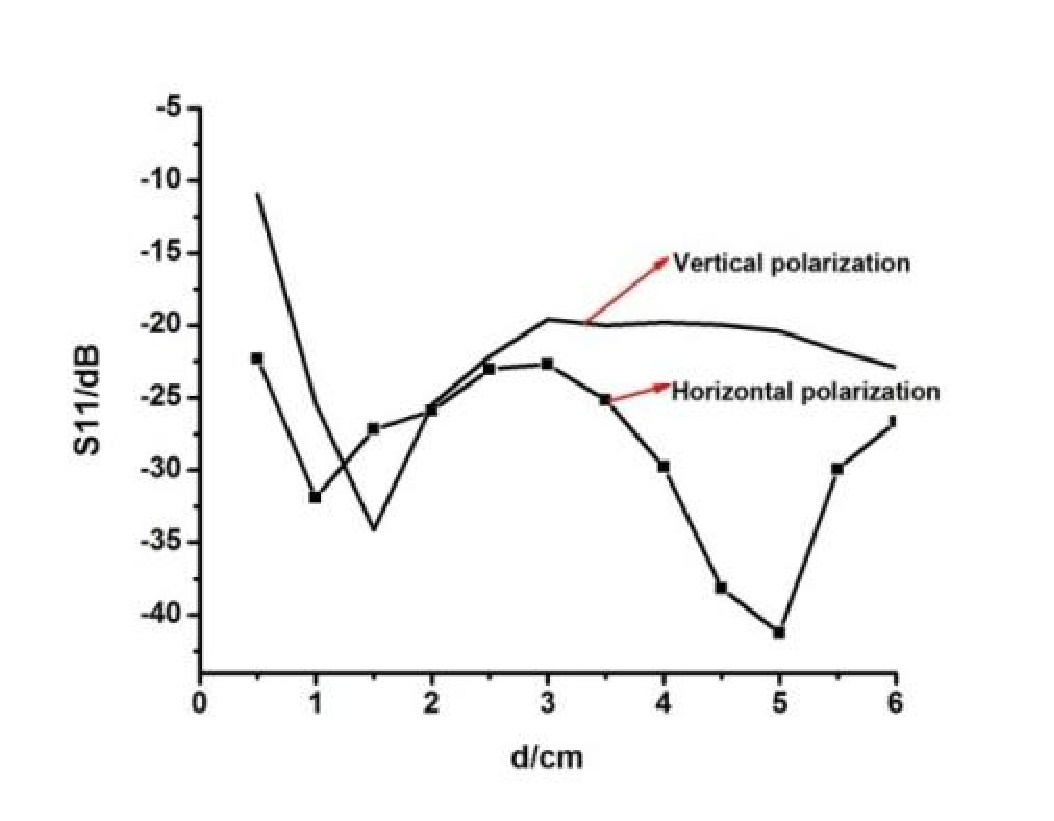
\includegraphics[width=\textwidth]{figs/5a.eps}
\caption{S11 changes}
\label{fig:5a}	
\end{subfigure}		
\begin{subfigure}[b]{0.4\textwidth}
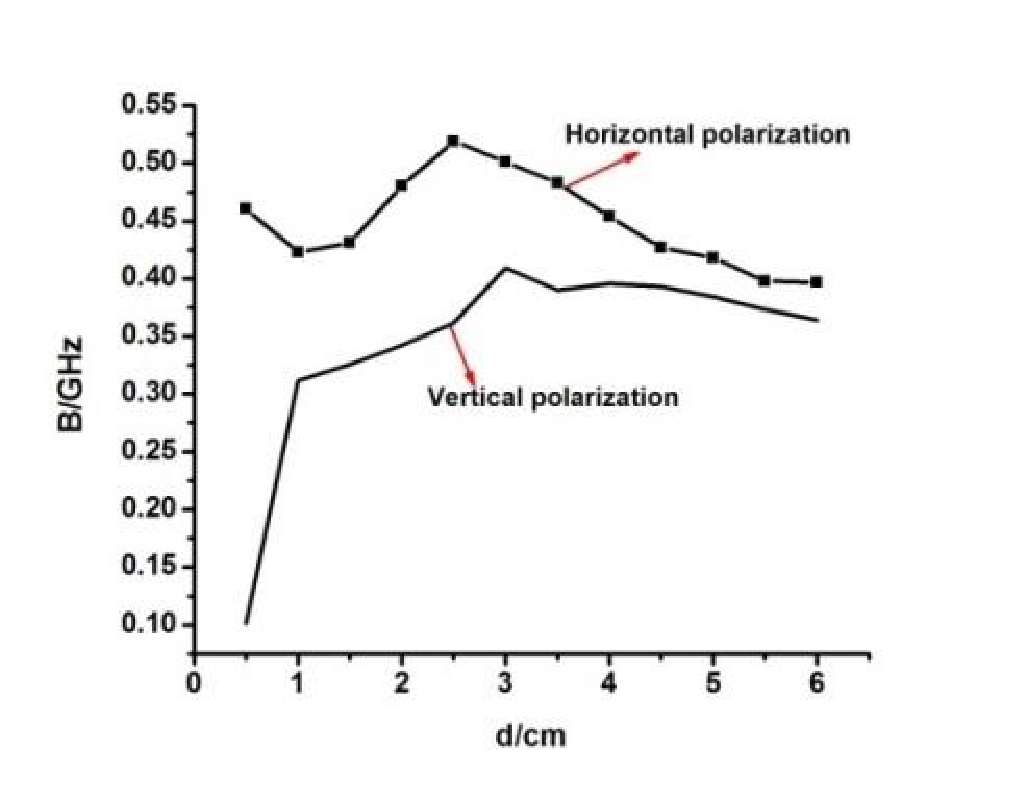
\includegraphics[width=\textwidth]{figs/5b.eps}
\caption{B changes}
\label{fig:5b}
\end{subfigure}
\caption{Comparison of S11 and \textit{B} of horizontal polarization and vertical polarization with different
\textit{d}}
\label{fig:5}
\end{figure}

\begin{figure}[!htb]
\centering
\begin{subfigure}[b]{0.24\textwidth}
\includegraphics[width=\textwidth]{figs/6a.pdf}
\caption{E(YZ) plane of horizontal polarization}
\label{fig:6a}	
\end{subfigure}		
\begin{subfigure}[b]{0.24\textwidth}
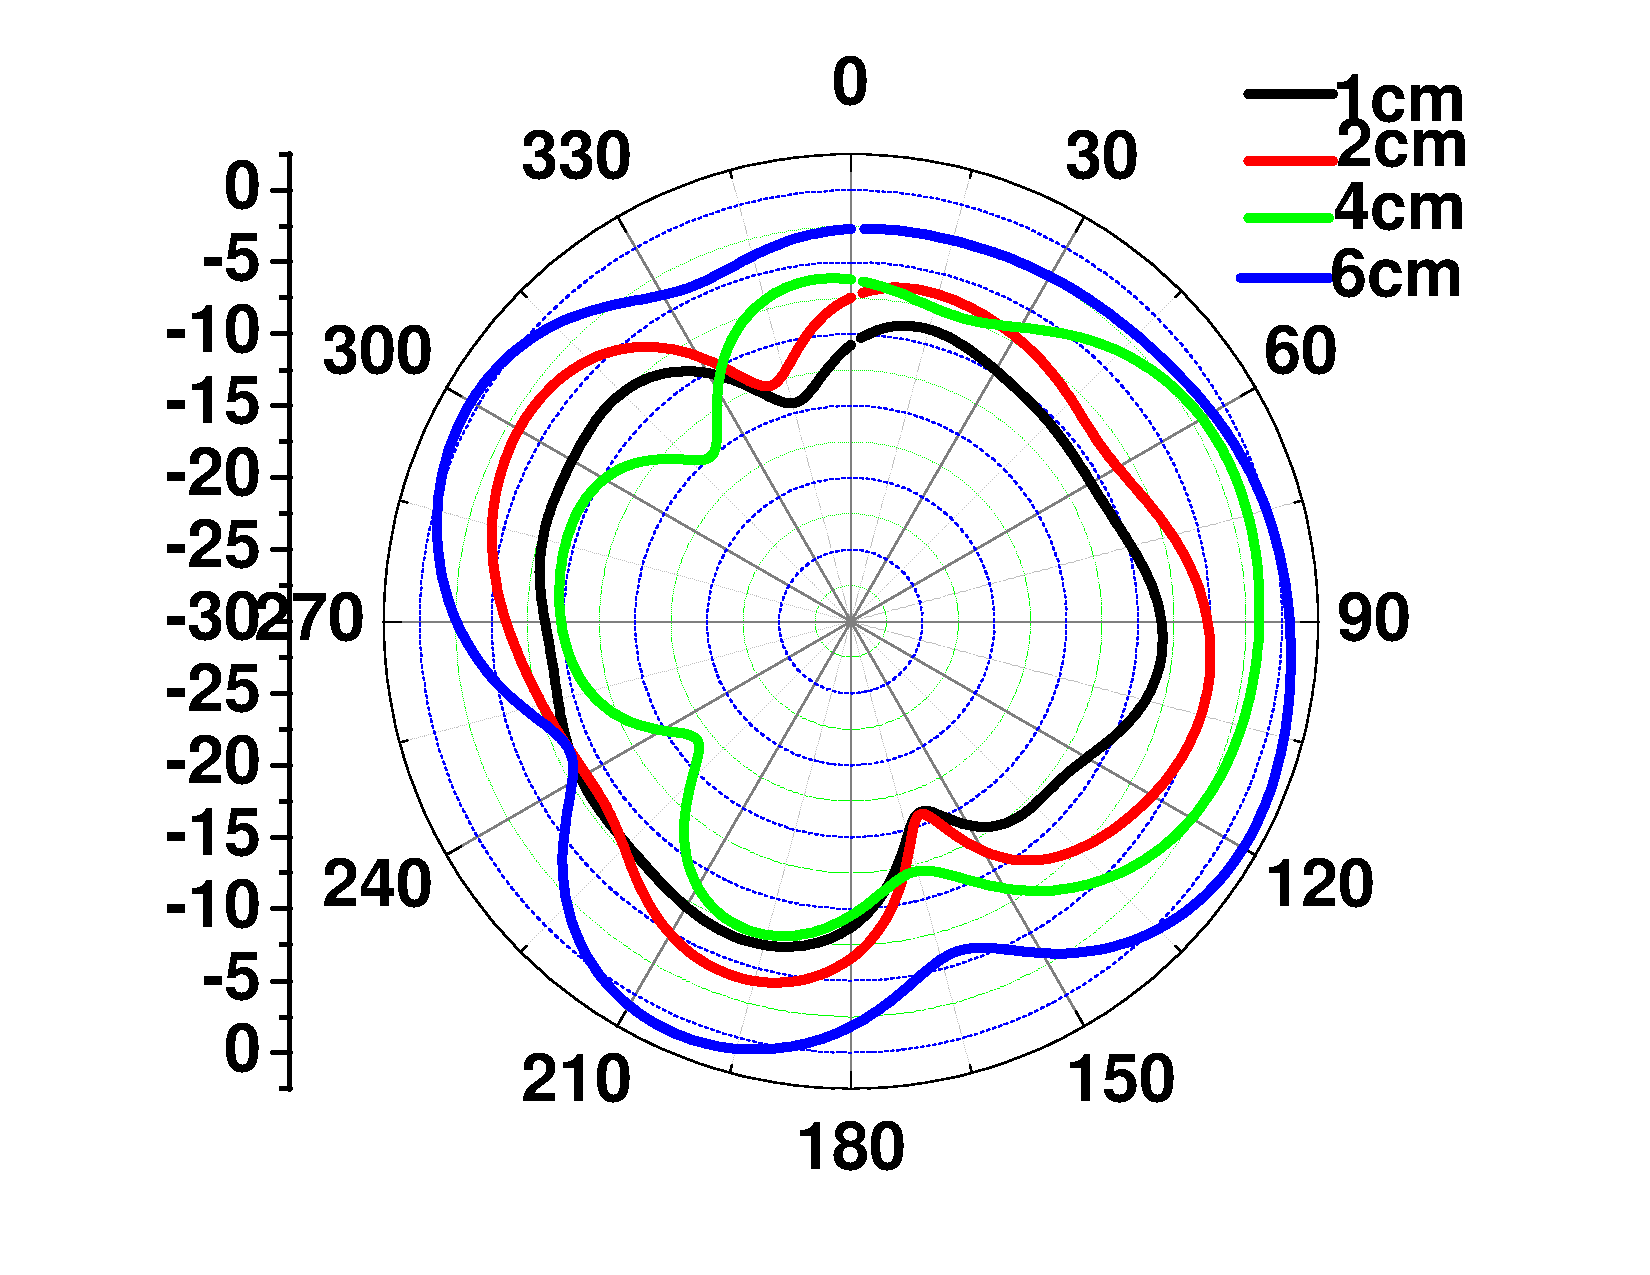
\includegraphics[width=\textwidth]{figs/6b.pdf}
\caption{E plane of vertical polarization}
\label{fig:6b}
\end{subfigure}
\begin{subfigure}[b]{0.24\textwidth}
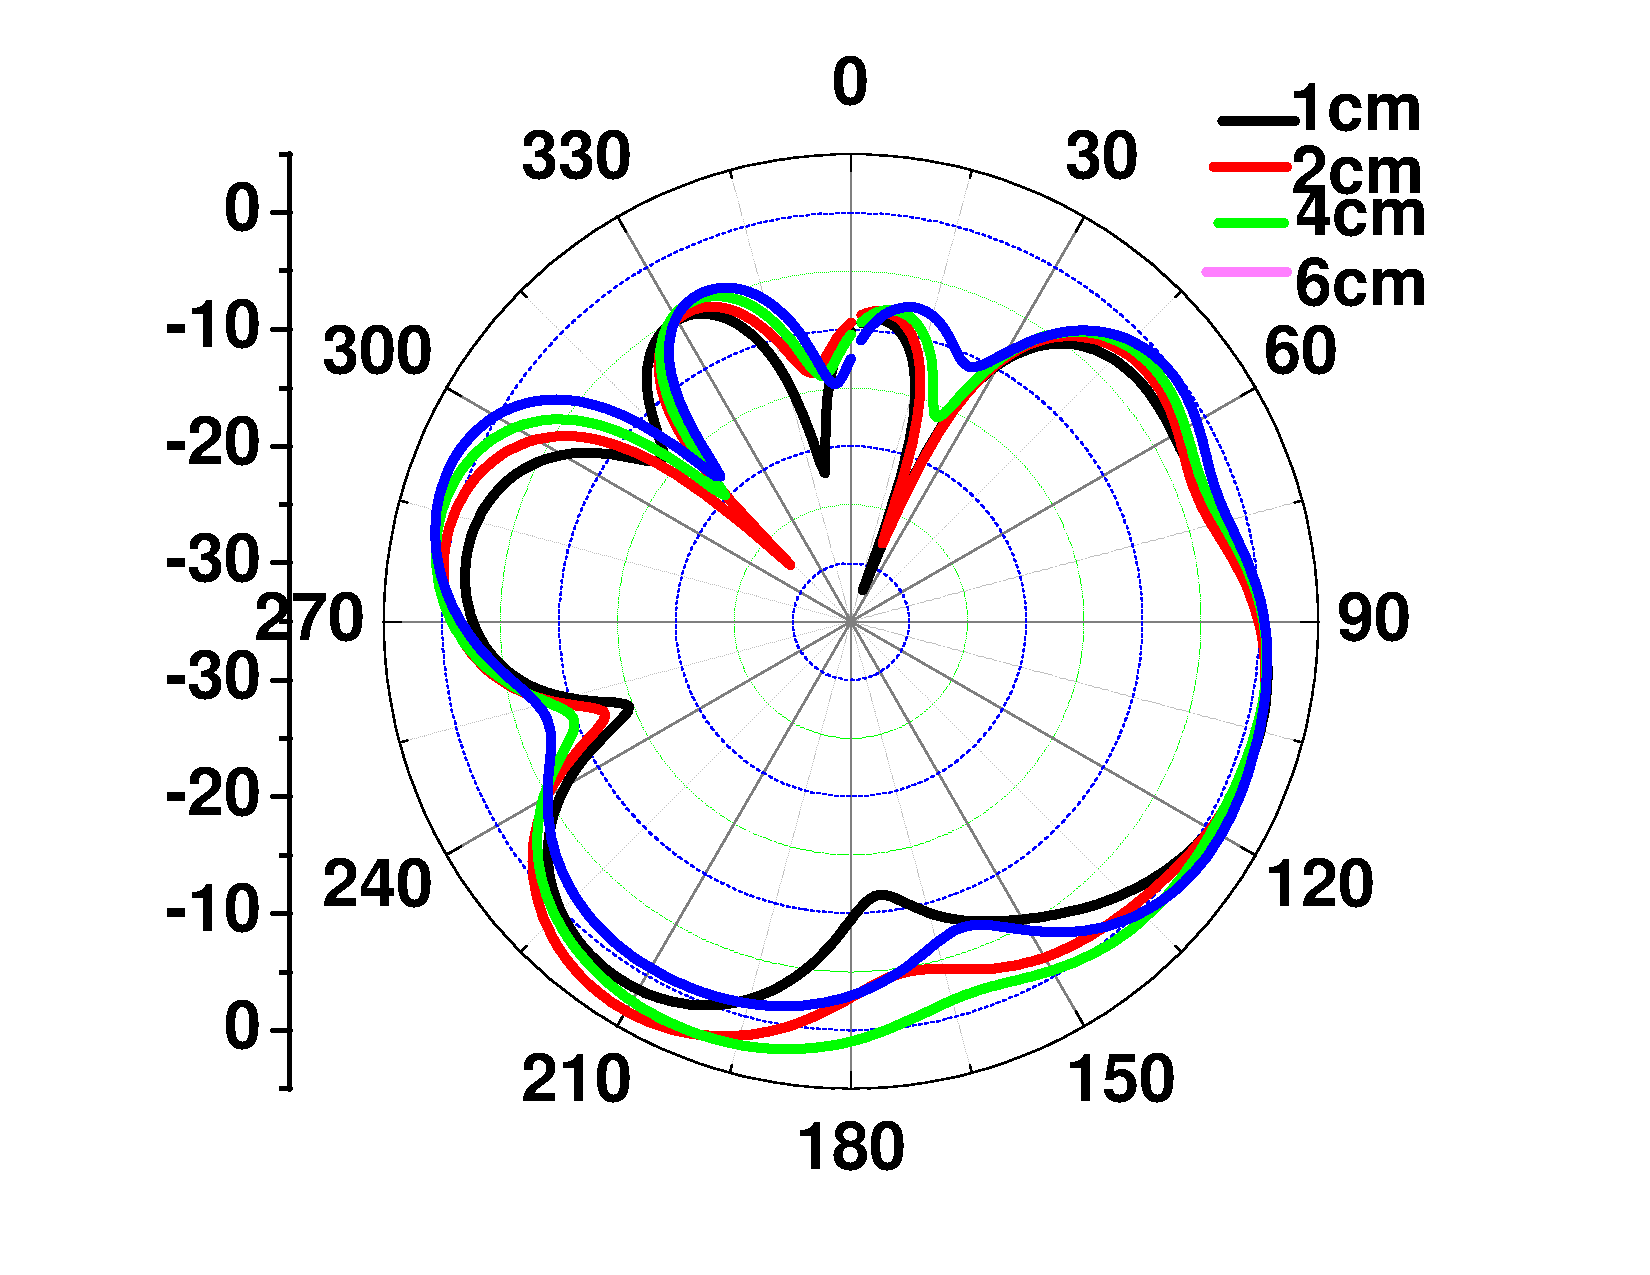
\includegraphics[width=\textwidth]{figs/6d.pdf}
\caption{H(XY) plane of horizontal polarization}
\label{fig:6d}	
\end{subfigure}
\begin{subfigure}[b]{0.24\textwidth}
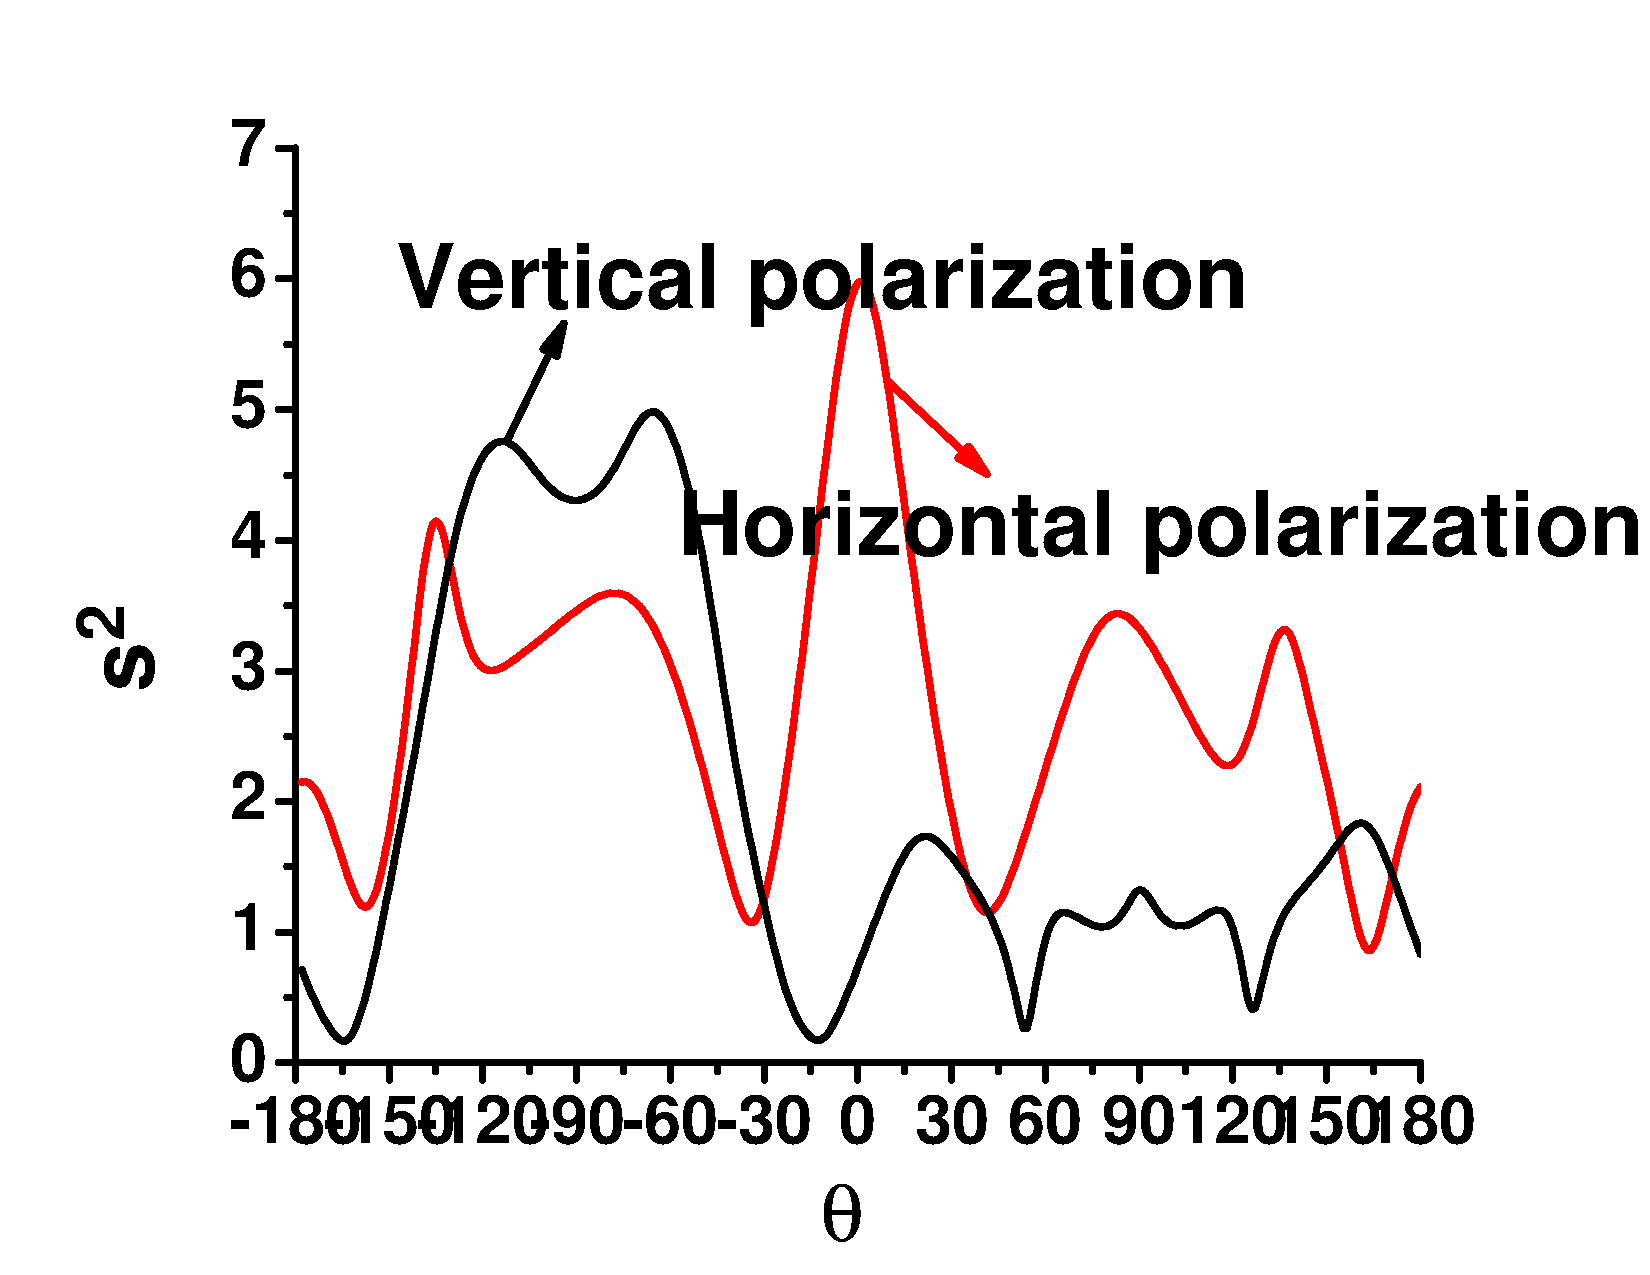
\includegraphics[width=\textwidth]{figs/6e.pdf}
\caption{H plane of vertical polarization}
\label{fig:6e}	
\end{subfigure}
\begin{subfigure}[b]{0.24\textwidth}
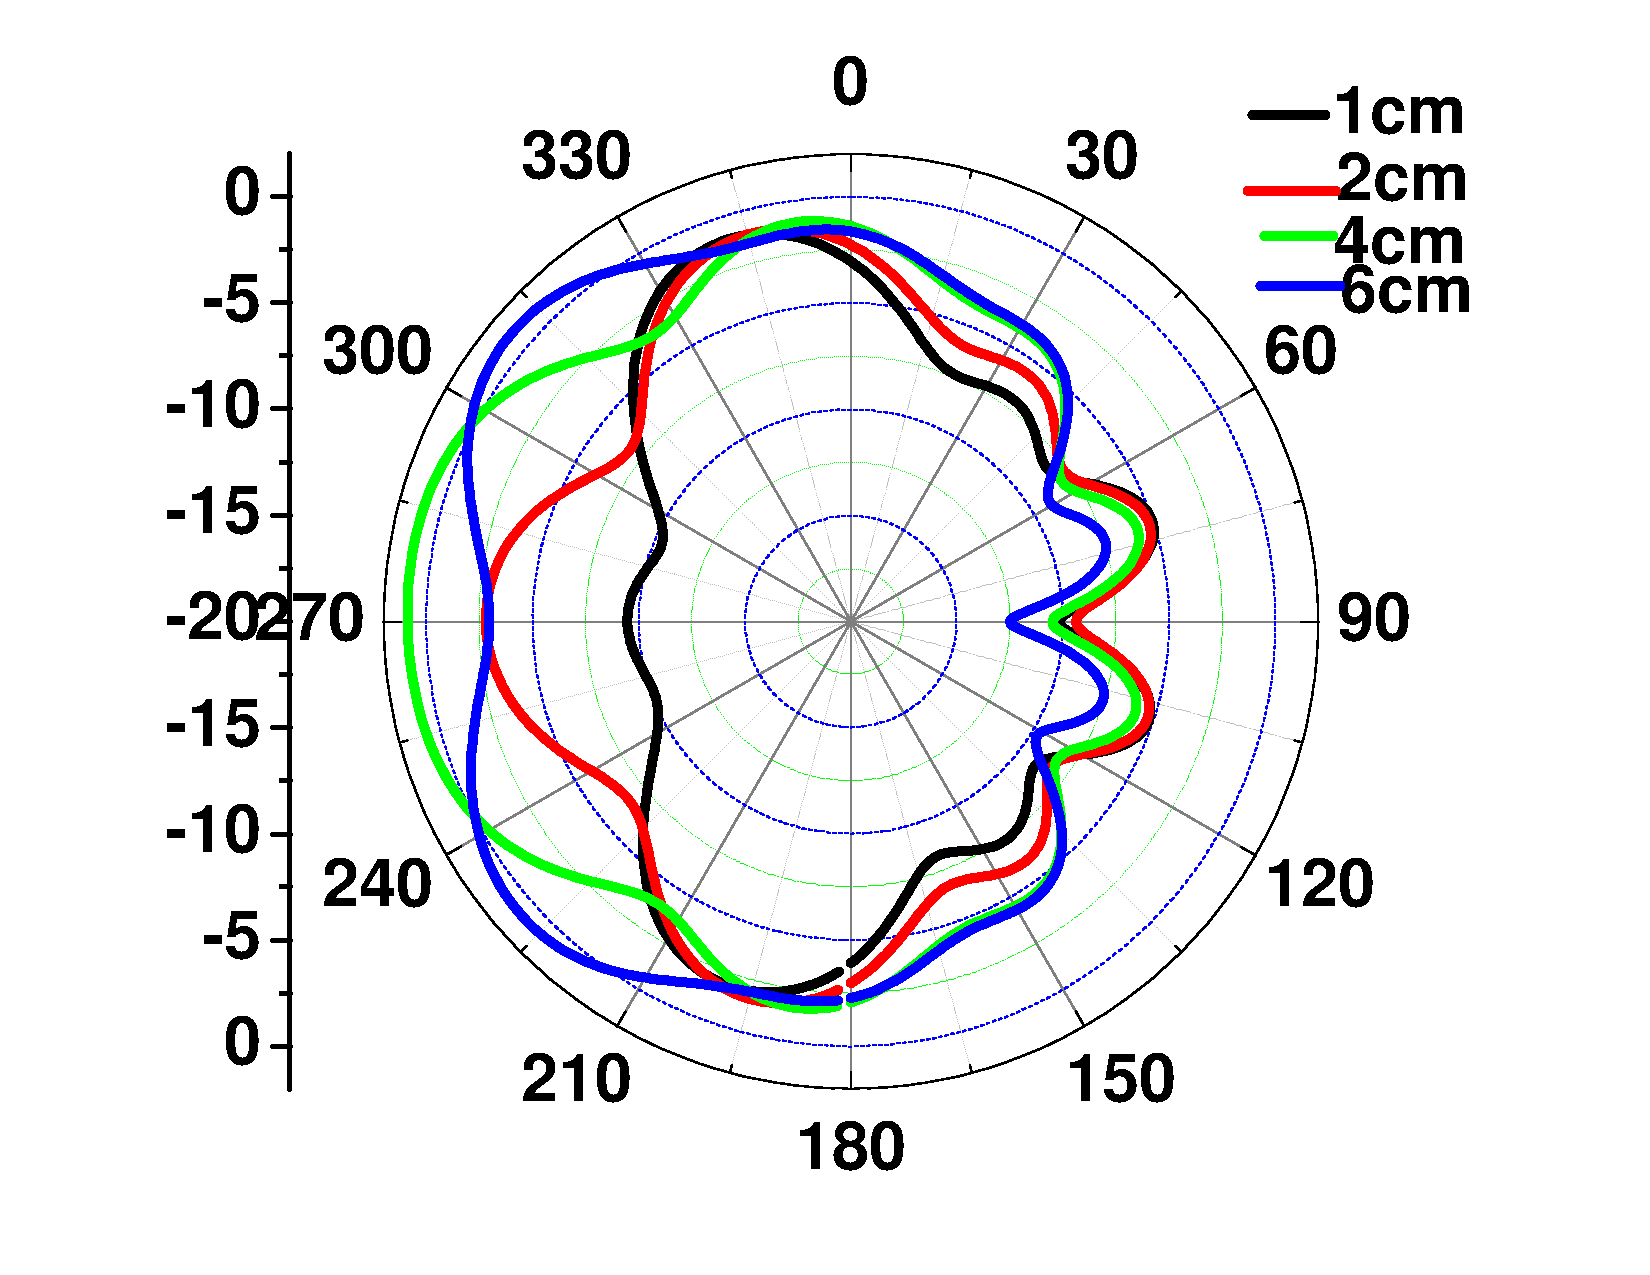
\includegraphics[width=\textwidth]{figs/6c.pdf}
\caption{E-plane}
\label{fig:6c}	
\end{subfigure}
\begin{subfigure}[b]{0.24\textwidth}
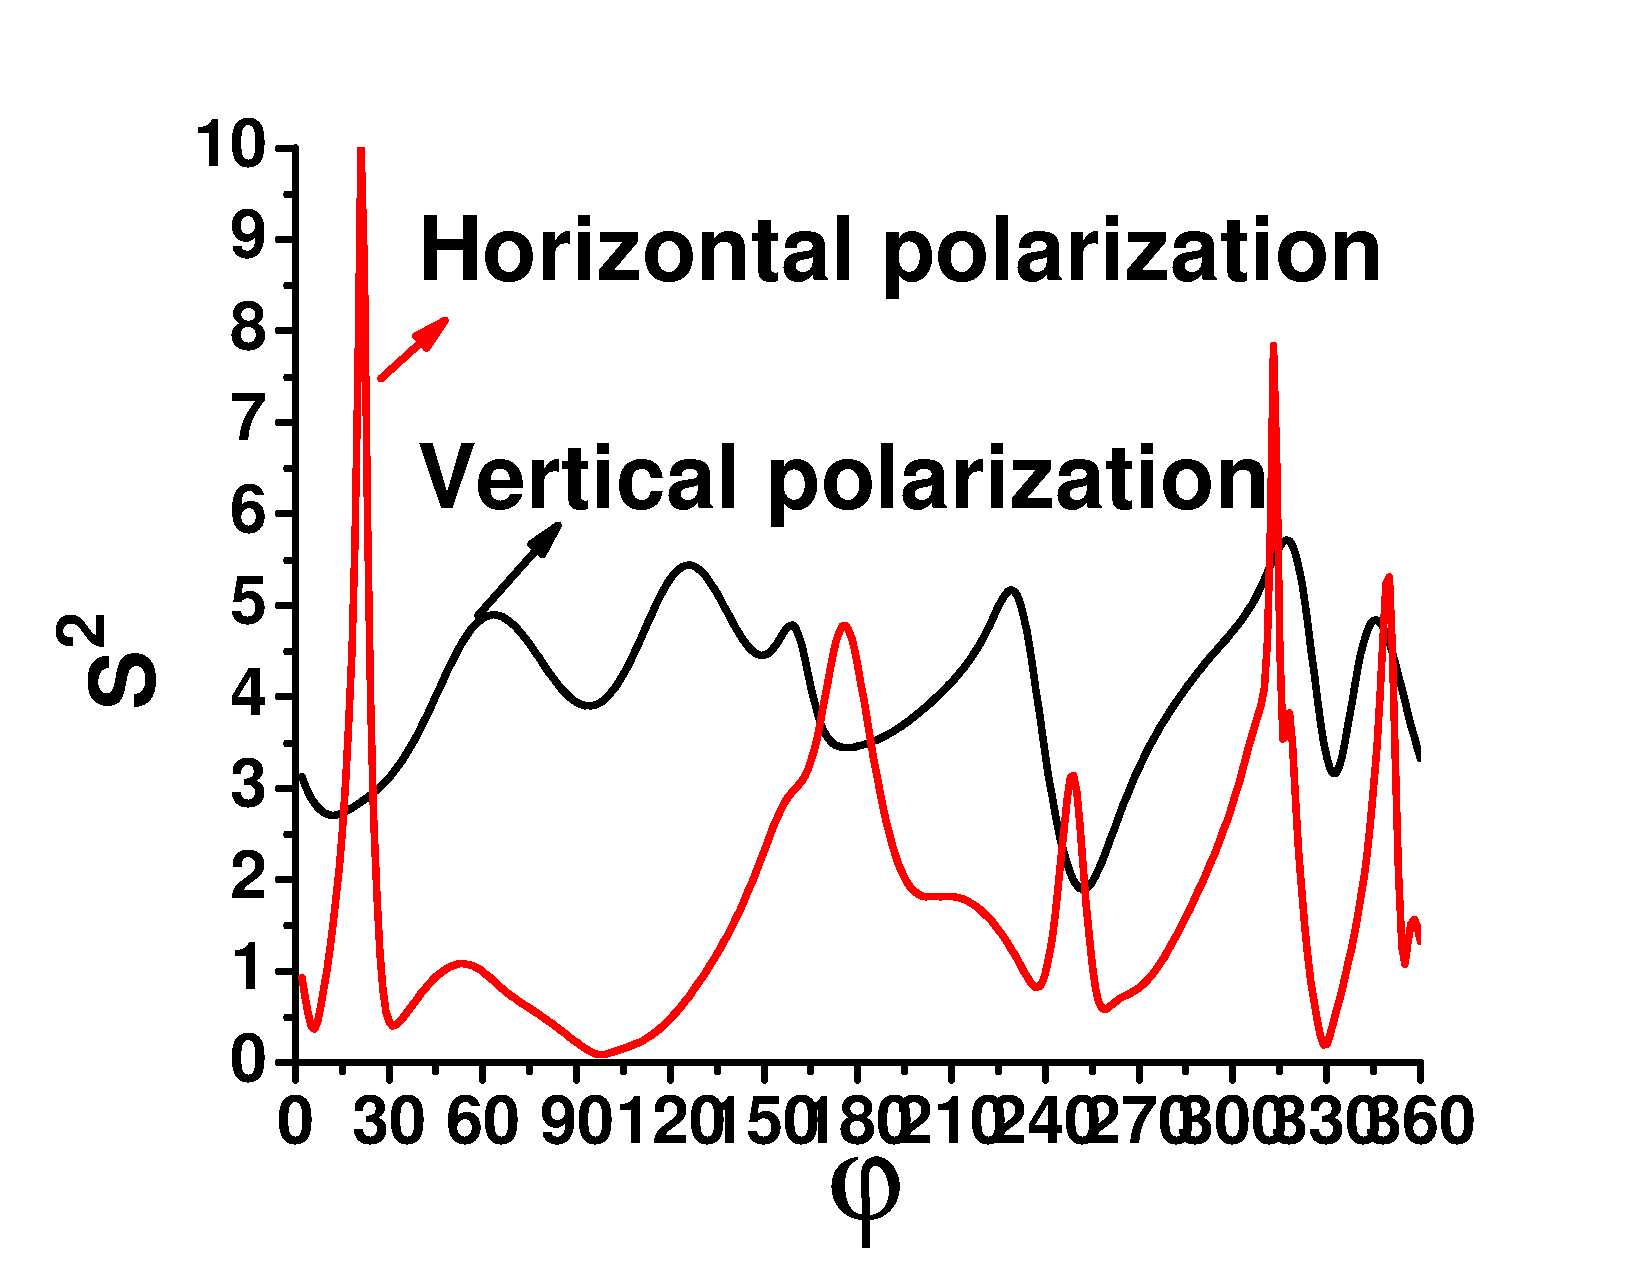
\includegraphics[width=\textwidth]{figs/6f.pdf}
\caption{H-plane}
\label{fig:6f}	
\end{subfigure}
\caption{Comparison of gain pattern of horizontal polarization and vertical polarization of \textit{d}.
$S^2= \frac{\sum_{d=1}^n{({G_b-G})^2}}{n}$ (d=1cm, 2cm, 4cm, 6cm) }
\label{fig:6}
\end{figure}
When \textit{d}=0.5cm, the bandwidth is the narrowest, and the antenna is not suitable for placing on body surface this time.
S11 of horizontal polarization decreases with the increase of d. When \textit{d}=5cm, S11 is the smallest and the antenna
matching is the best; When 0.5cm\textless\textit{d}\textless1.5cm, S11 of vertical polarization decreases with the increase of
\textit{d} and when \textit{d}=1.5cm, S11 reaches the minimum and the antenna matching performance is the best, when
1.5cm$<\textit{d}<$4cm, S11 increases with the increase of d, and the antenna matching performance get worse. When
0.5cm$<\textit{d}<$1.2cm, \textit{d}\textgreater2cm, the horizontal polarization of S11 is always smaller than vertical
polarization and the bandwidth is always wider than vertical polarization. Therefore, horizontal polarization of the antenna
performance is better than vertical polarization of this range of \textit{d}.
\begin{figure}[!htb]
\centering
\begin{subfigure}[b]{0.24\textwidth}
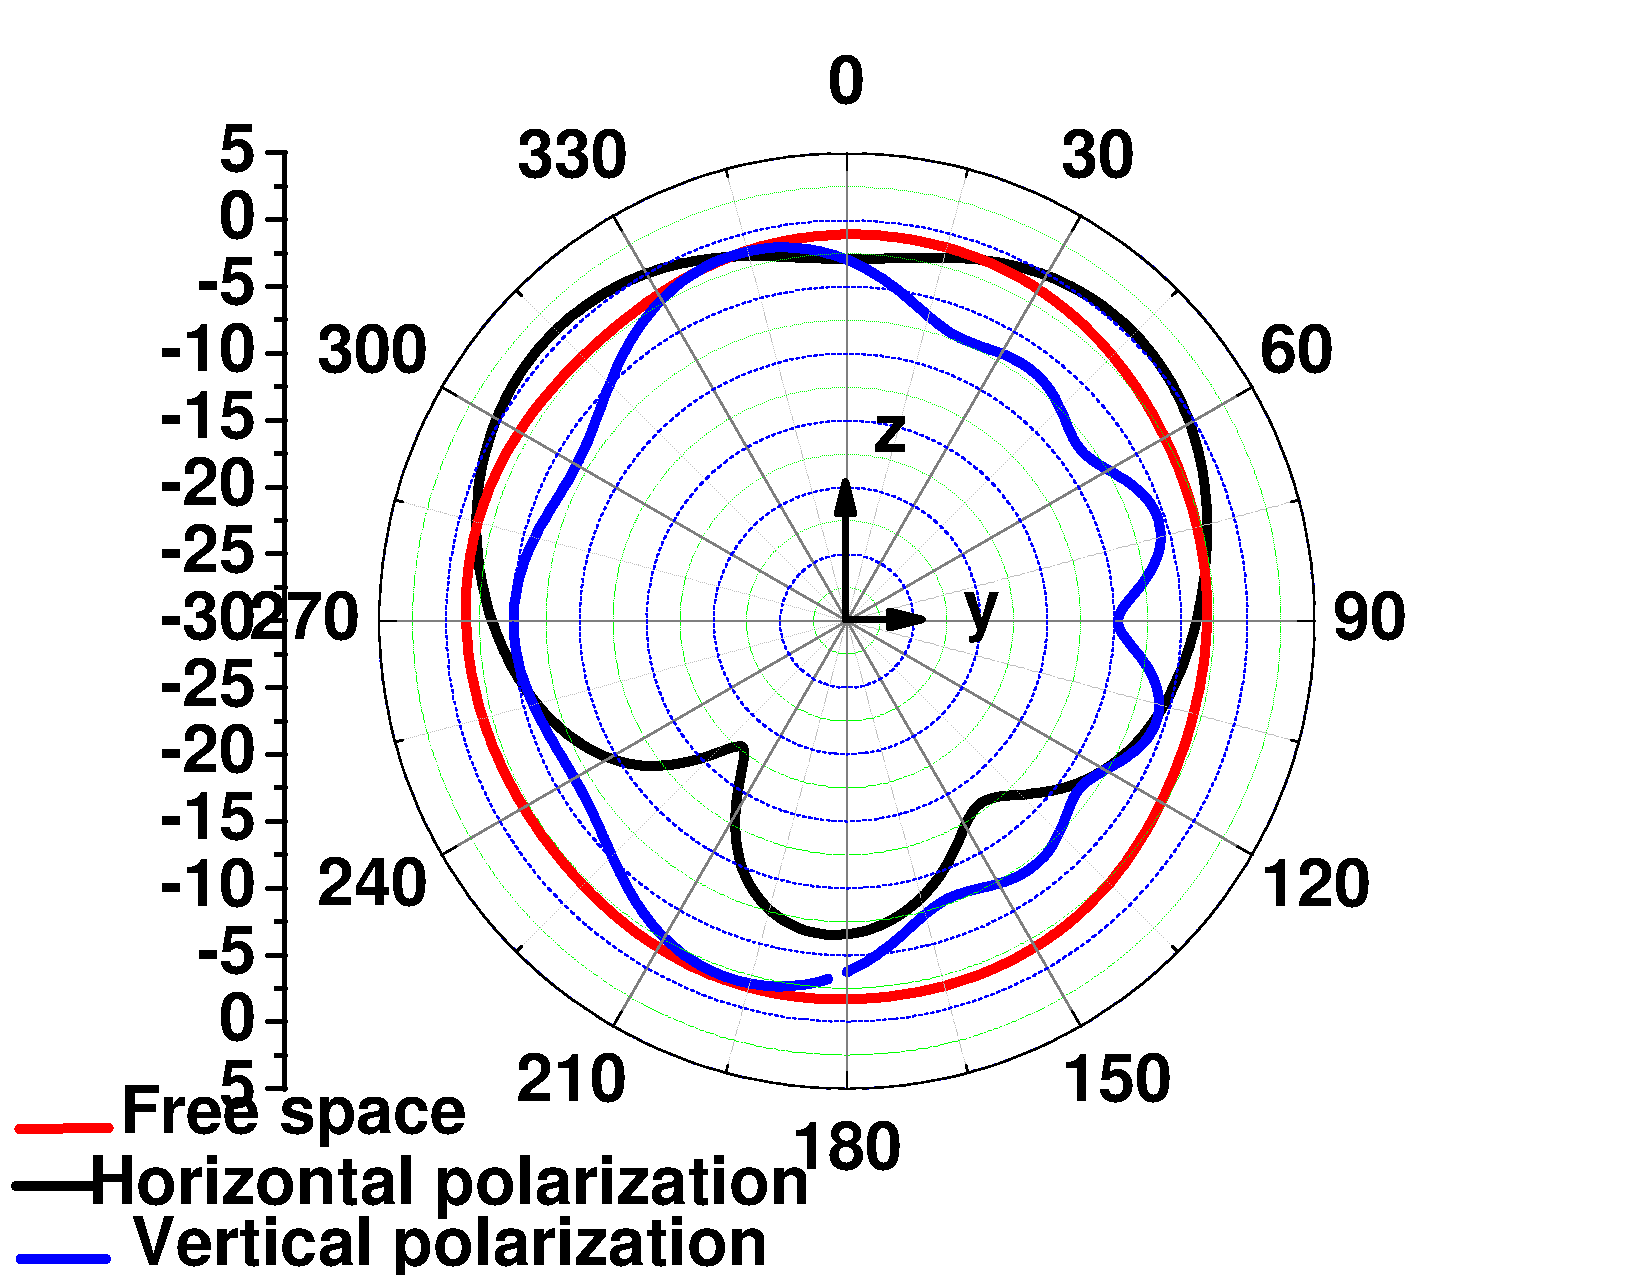
\includegraphics[width=\textwidth]{figs/7a.pdf}
\caption{E-plane}
\label{fig:7a}	
\end{subfigure}
\begin{subfigure}[b]{0.24\textwidth}
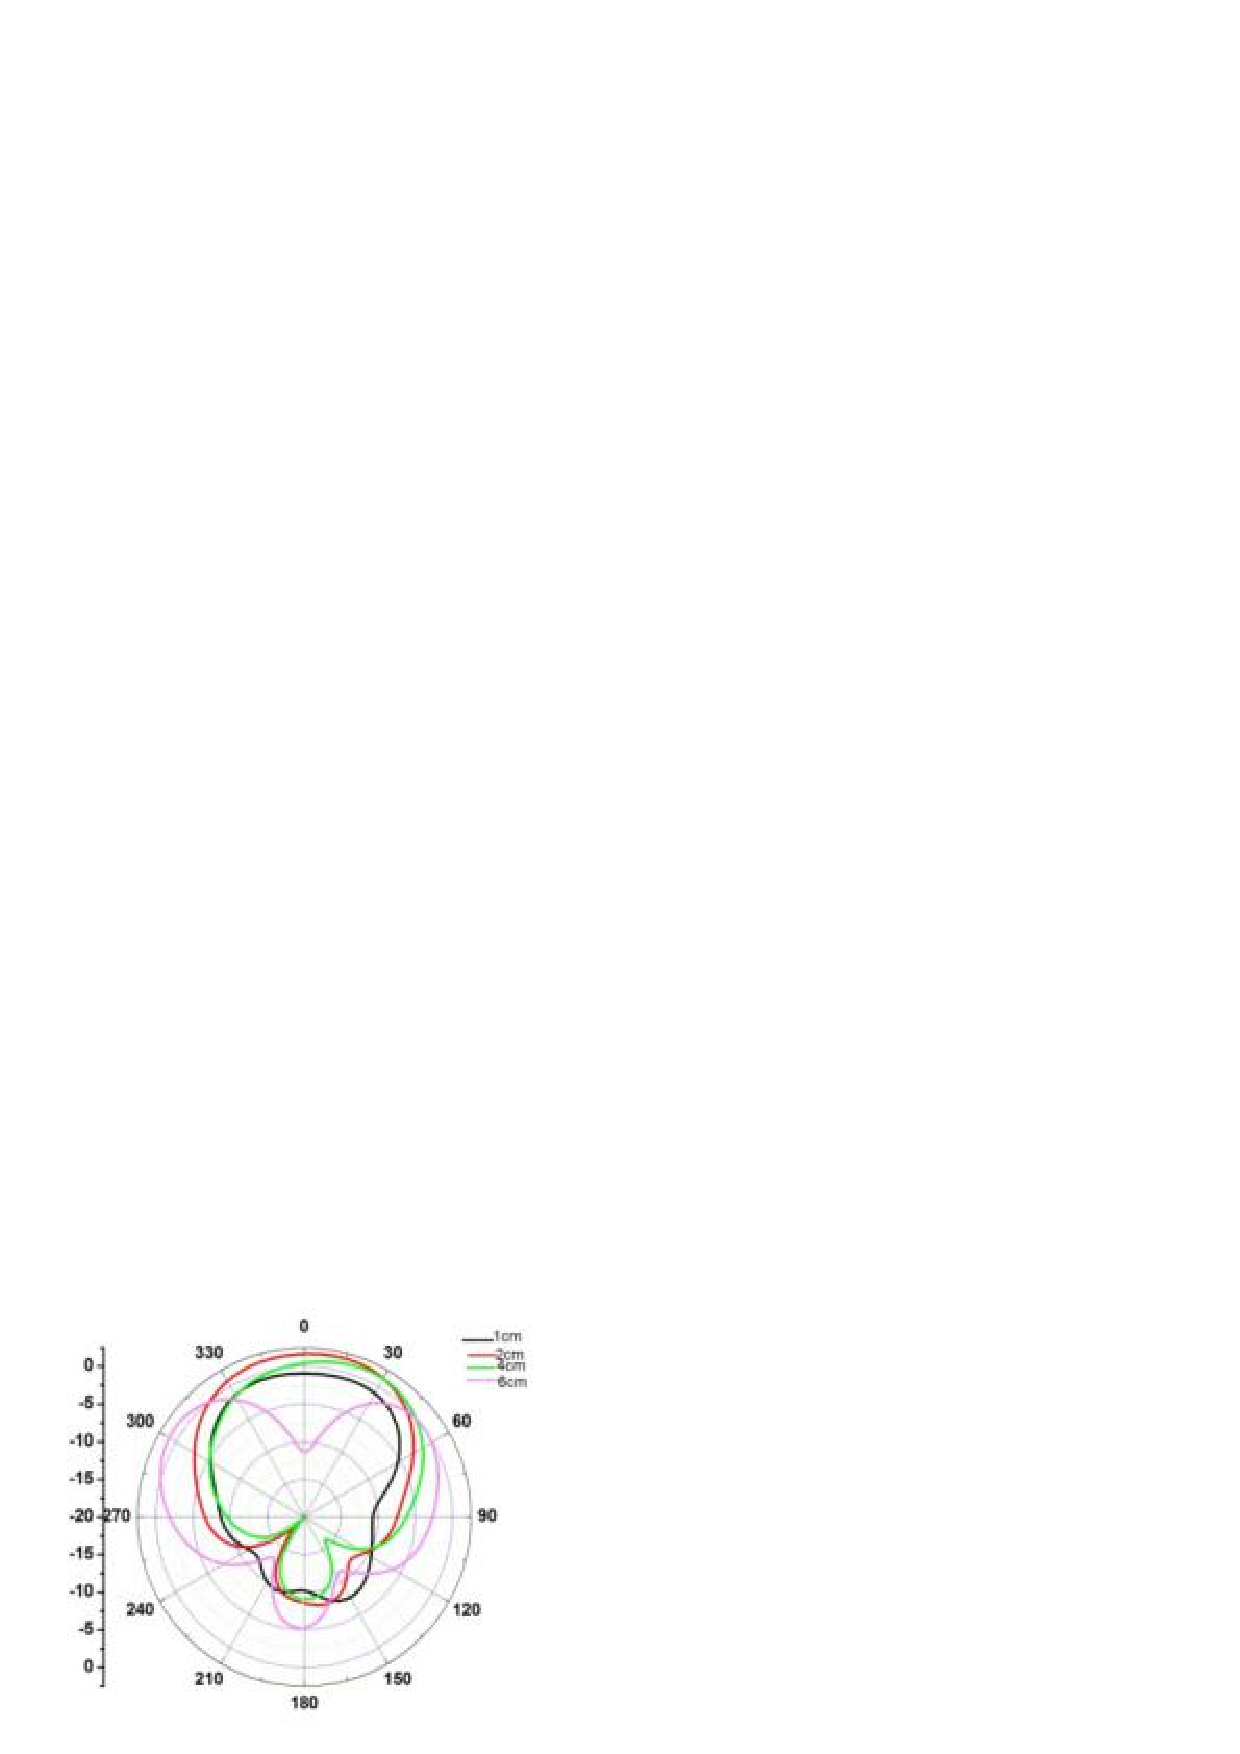
\includegraphics[width=\textwidth]{figs/7b.pdf}
\caption{H-plane}
\label{fig:7c}	
\end{subfigure}		
\begin{subfigure}[b]{0.23\textwidth}
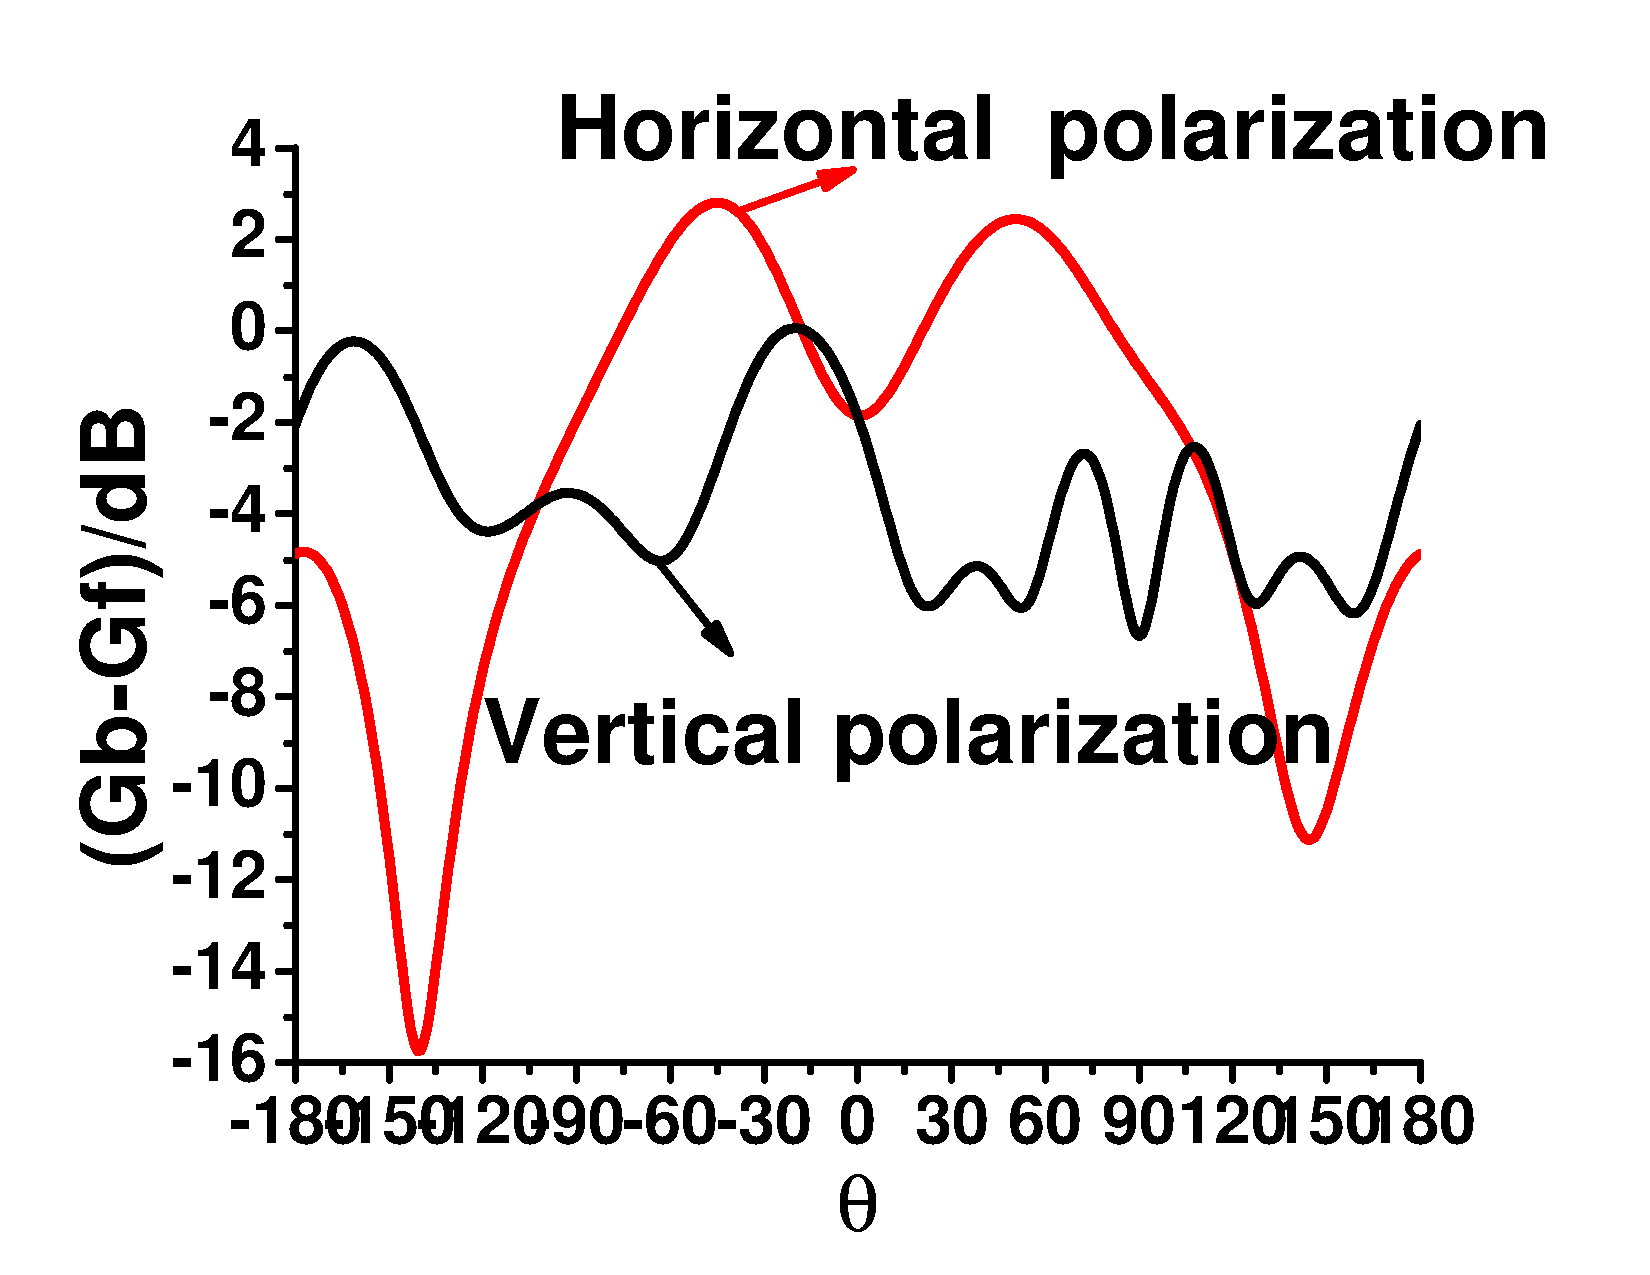
\includegraphics[width=\textwidth]{figs/7c.pdf}
\caption{Differential gain of E-plane }
\label{fig:7b}
\end{subfigure}
\begin{subfigure}[b]{0.23\textwidth}
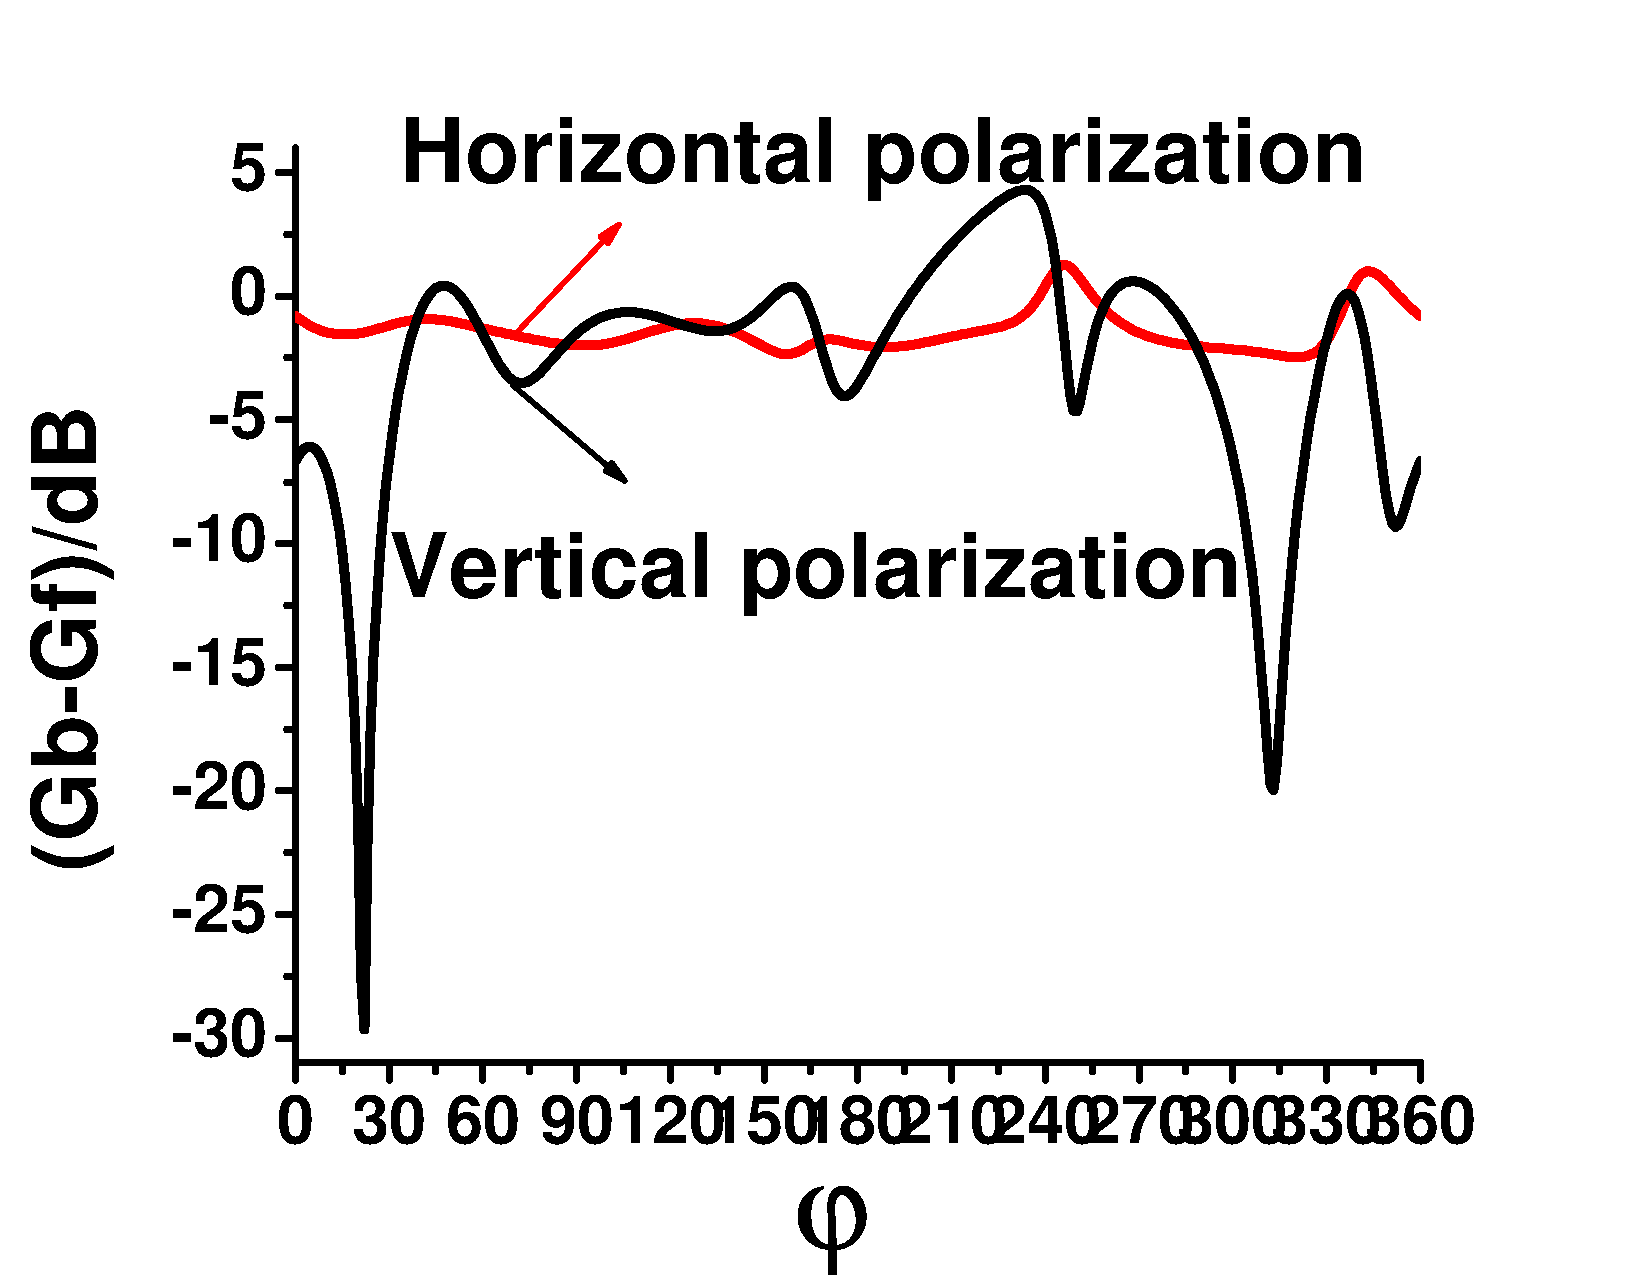
\includegraphics[width=\textwidth]{figs/7d.pdf}
\caption{Differential gain of H-plane}
\label{fig:7d}	
\end{subfigure}
\caption{Gain pattern of IFA. $G_{b}$: Gain of antenna on body surface, $G_{f}$: Gain of antenna in free space }
\label{fig:7}
\end{figure}

As shown in Fig. \ref{fig:6}, E-plane pattern of horizontal polarization is stable and not sensitive to \textit{d}. For H-plane pattern, when
$0\,^{\circ}$\textless$\varphi$\textless$30\,^{\circ}$, $310\,^{\circ}$��\textless$\varphi$\textless$330\,^{\circ}$,
$S^{2}$\textgreater5, indicating that the difference between the gain in the same direction is great and antenna directional
gain is sensitive to distance. The directional gain distribution of vertical polarization at different distances is relatively
uniform and not sensitive to the \textit{d}.

By comparing the antenna polarization performance at different distances, it��s found that the impact on antenna is not obvious
of \textit{d}. Therefore, 5cm and 1.5cm are selected as the research focus for horizontal polarization and vertical
polarization, respectively.
E-plane radiation pattern of horizontal polarization and vertical polarization after loading body model are symmetrical
distribution of $\theta$=$0\,^{\circ}$ and $\theta$=$90\,^{\circ}$ as shown in Fig. \ref{fig:7}. The fitted gain difference curve equation of horizontal
polarization is
\begin{equation}
\label{eq:eps_2}
y[dB]=0.0003797+0.00488x+1.00823,  x[cm]
\end{equation}
The  body model has a great influence on the antenna gain at the position of
$-180\,^{\circ}$\textless$\theta$\textless$-125\,^{\circ}$, $125\,^{\circ}$��\textless$\theta$\textless$180\,^{\circ}$, and
when $\theta$=$140\,^{\circ}$, $\mid$$G_{b}$-$G_{f}$$\mid$ is the maximum and the human body has the most obvious effects on
antenna. For vertical polarization, $\mid$$G_{b}$-$G_{f}$$\mid$\textless6, human body has a uniform effect on antenna gain
pattern over the entire range of \textit{$\theta$}. The impact of human body to vertical polarization are more obvious than
horizontal polarization.\\
H-plane pattern of horizontal polarization after loading body model is similar to omnidirectional distribution of free space.
For vertical polarization, when $0\,^{\circ}$\textless$\varphi$\textless$35\,^{\circ}$,
$295\,^{\circ}$\textless$\varphi$\textless$320\,^{\circ}$, $340\,^{\circ}$\textless$\varphi$\textless$360\,^{\circ}$,
$\mid$$G_{b}$-$G_{f}$$\mid$\textgreater4, human body has great effects on antenna gain pattern, when $\varphi$=$17\,^{\circ}$,
$\mid$$G_{b}$-$G_{f}$$\mid$ reach the maximum and human body has the most obvious effects on antenna.
\subsection{MIFA}
\begin{figure}[!htb]
\centering
\begin{subfigure}[b]{0.4\textwidth}
\includegraphics[width=\textwidth]{figs/8a.eps}
\caption{S11 changes}
\label{fig:8a}	
\end{subfigure}		
\begin{subfigure}[b]{0.4\textwidth}
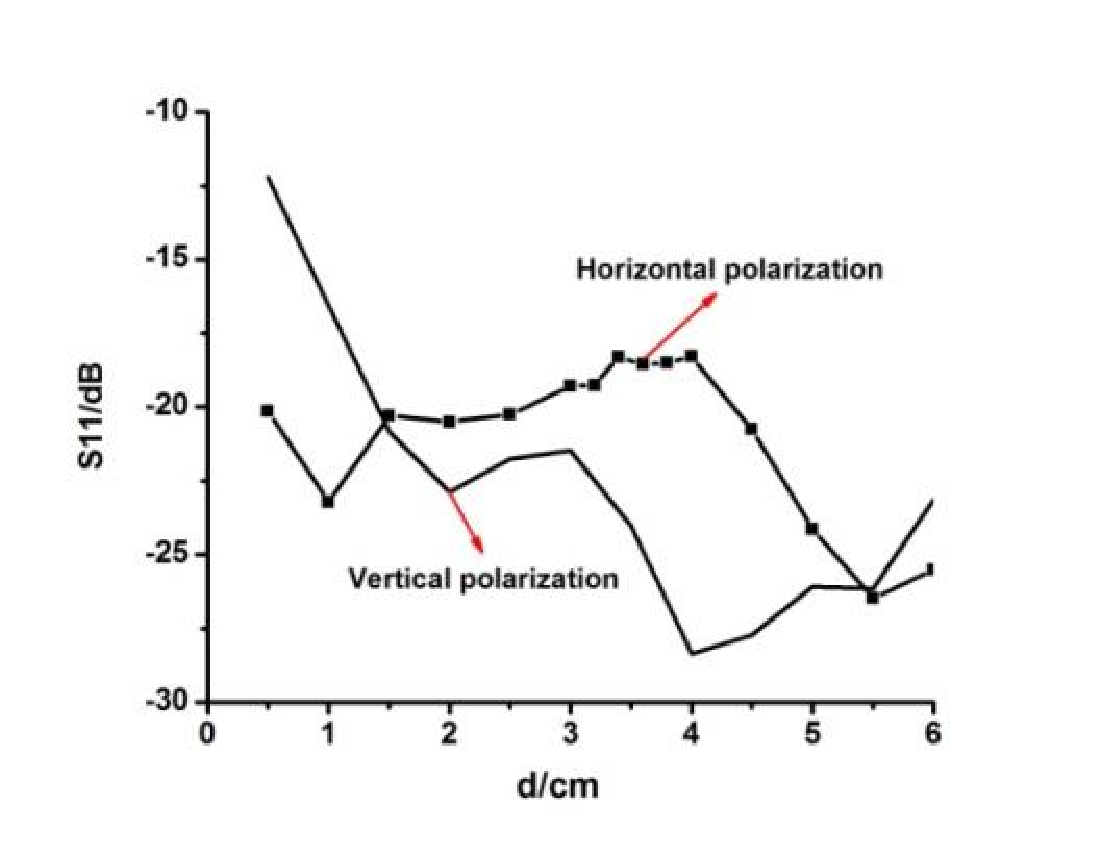
\includegraphics[width=\textwidth]{figs/8b.eps}
\caption{B changes}
\label{fig:8b}
\end{subfigure}
\caption{Comparison of S11 and B of horizontal polarization and vertical polarization with different \textit{d}}
\label{fig:8}
\end{figure}
For horizontal polarization, the fitting equation for bandwidth is
\begin{equation}
\label{eq:eps_3}
y[GHz]=-0.00178x^2+0.01416x+0.18396,  x[cm]
\end{equation}
When \textit{d}=1.5cm, the bandwidth is the narrowest, and the antenna is not suitable for placing on body surface. For
horizontal polarization, the effect of distance on bandwidth is not obvious. When \textit{d}=1cm, \textit{B}=225GHz, reaching
the maximum. The fitting equation for S11 of vertical polarization is
\begin{equation}
\label{eq:eps_4}
y[dB]=2.02866x-16.01,  x[cm]
\end{equation}
\begin{figure}[!htb]
\centering
\begin{subfigure}[b]{0.24\textwidth}
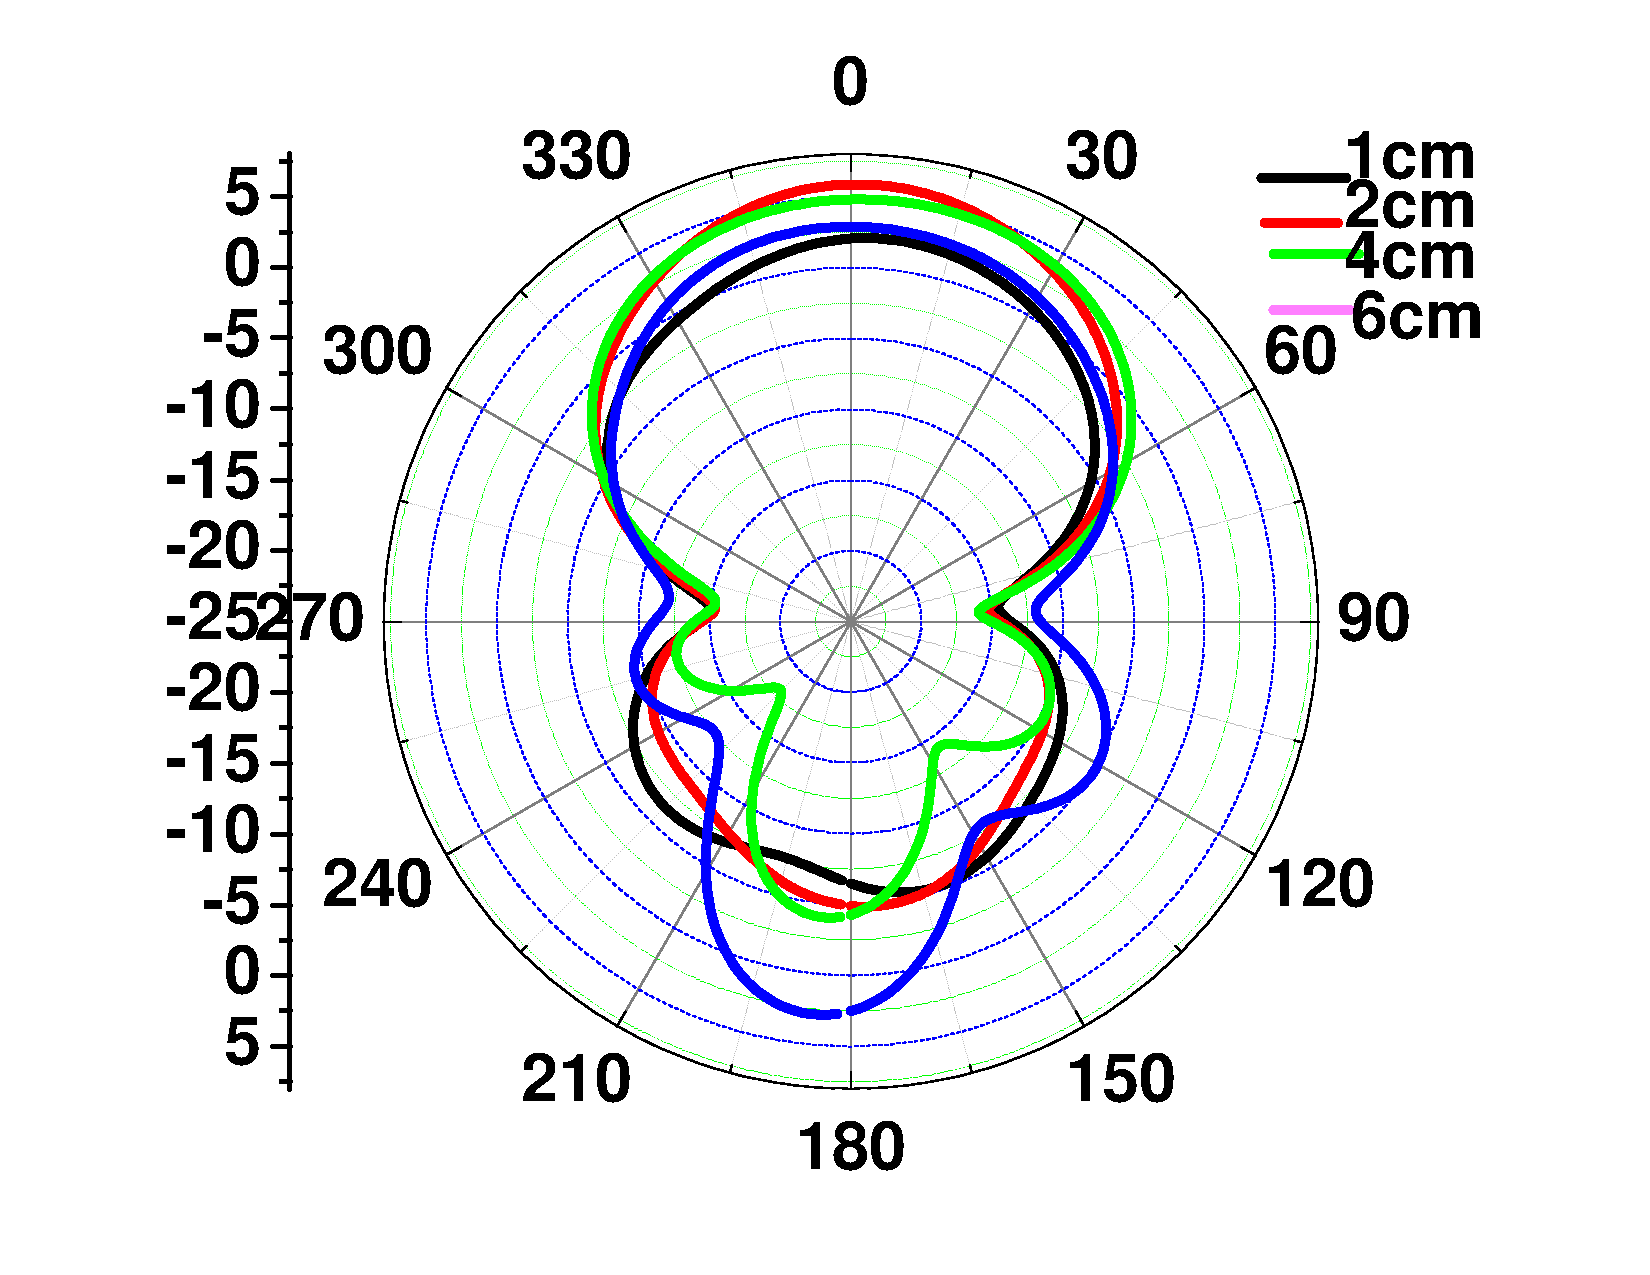
\includegraphics[width=\textwidth]{figs/9a.pdf}
\caption{Horizontal polarization of E-plane}
\label{fig:9a}	
\end{subfigure}		
\begin{subfigure}[b]{0.24\textwidth}
\includegraphics[width=\textwidth]{figs/9b.pdf}
\caption{Vertical polarization of E-plane }
\label{fig:9b}
\end{subfigure}
\begin{subfigure}[b]{0.24\textwidth}
\includegraphics[width=\textwidth]{figs/9c.pdf}
\caption{Horizontal polarization of H-plane}
\label{fig:9d}	
\end{subfigure}
\begin{subfigure}[b]{0.24\textwidth}
\includegraphics[width=\textwidth]{figs/9d.pdf}
\caption{Vertical polarization of H-plane}
\label{fig:9e}	
\end{subfigure}
\begin{subfigure}[b]{0.24\textwidth}
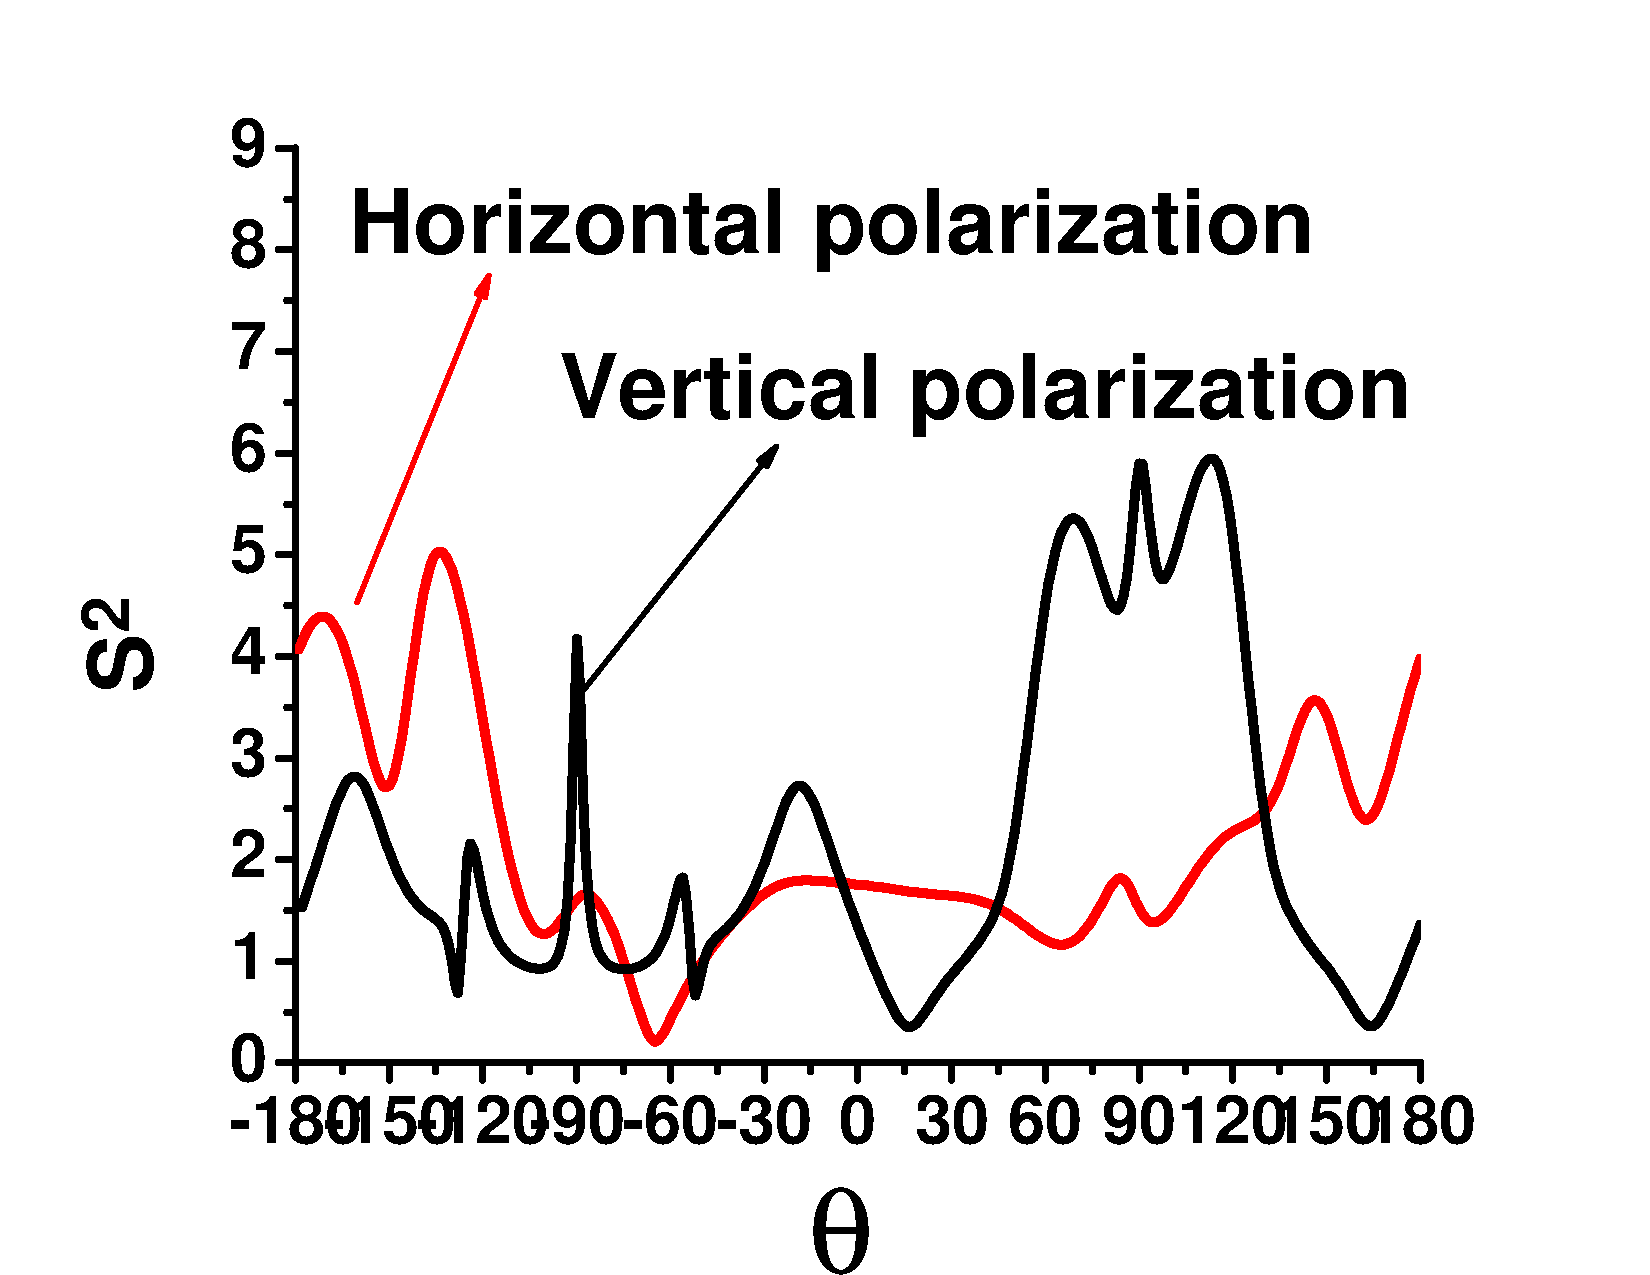
\includegraphics[width=\textwidth]{figs/9e.pdf}
\caption{E-plane}
\label{fig:9c}	
\end{subfigure}
\begin{subfigure}[b]{0.24\textwidth}
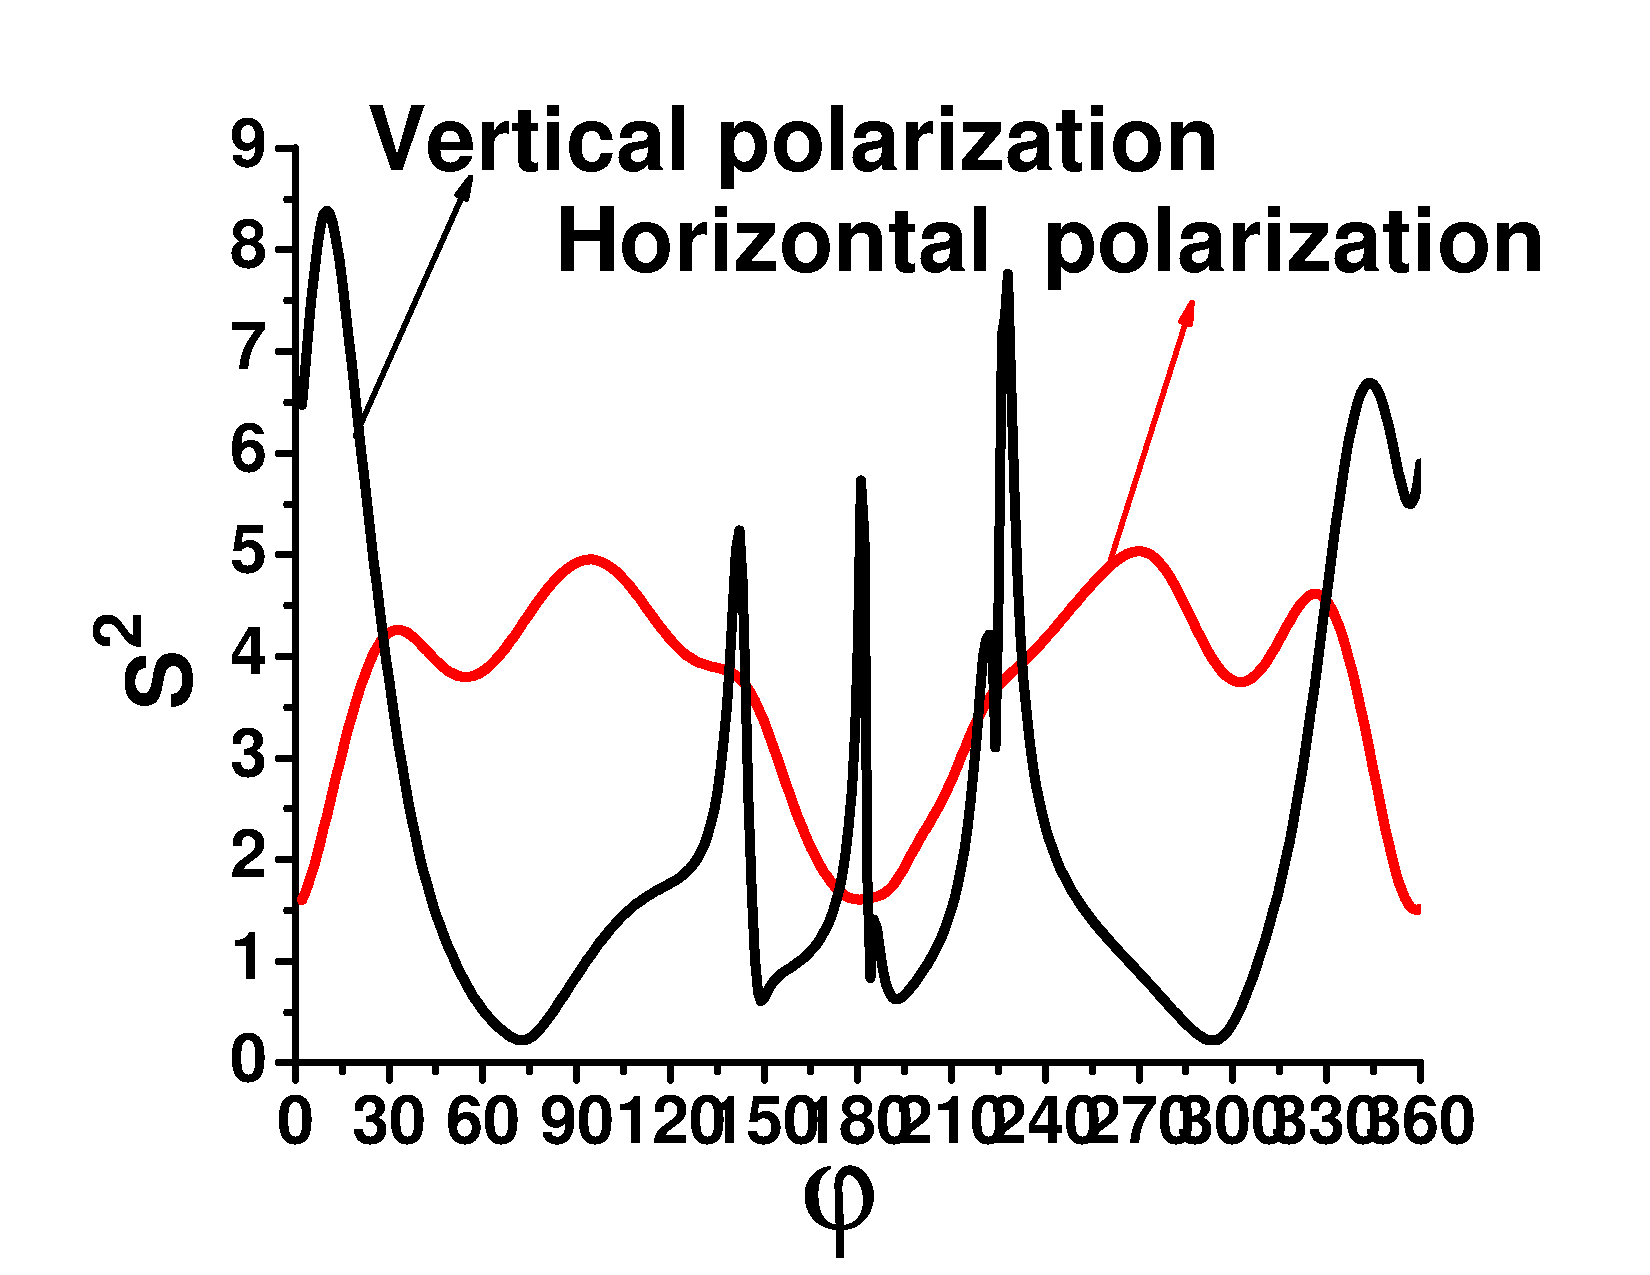
\includegraphics[width=\textwidth]{figs/9f.pdf}
\caption{H-plane}
\label{fig:9f}	
\end{subfigure}
\caption{Directional gain changes at different distances}
\label{fig:9}
\end{figure}
When \textit{d}=5.5cm, S11 takes the minimum. When 1cm$<\textit{d}<$2.5cm, S11 of vertically polarized is always smaller than
horizontal polarization, and the bandwidth is always wider than horizontal polarization. In this range, the antenna is more
suitable for placing on the surface of the human body in vertically polarized. When \textit{d}=0.5cm, S11 of vertical
polarization take the maximum and the bandwidth is the narrowest, so the antenna is not suitable for placing on human body
surface. The S11 curve of horizontal polarization is flat and when \textit{d}=4cm, \textit{B} reaches the maximum, so the
antenna is most suitable to place on human body surface.

For the horizontal polarization, the square gain distributions at different distances are relatively uniform and not sensitive
to distance. For E-plane pattern of vertical polarization, when $30\,^{\circ}$\textless$\varphi$\textless$150\,^{\circ}$,
$S^{2}$\textgreater4, The gain difference at different distances is relatively large, the antenna direction gain is more
sensitive to the distance factor than the other position. For H-plane pattern, when
$130\,^{\circ}$\textless$\varphi$\textless$180\,^{\circ}$, $0\,^{\circ}$\textless$\varphi$\textless$30\,^{\circ}$,
$225\,^{\circ}$\textless$\varphi$\textless$240\,^{\circ}$, $330\,^{\circ}$\textless$\varphi$\textless$360\,^{\circ}$,
$S^{2}$\textgreater4, the antenna direction gain is more sensitive to the distance factor.
\begin{figure}[!htb]
\centering
\begin{subfigure}[b]{0.24\textwidth}
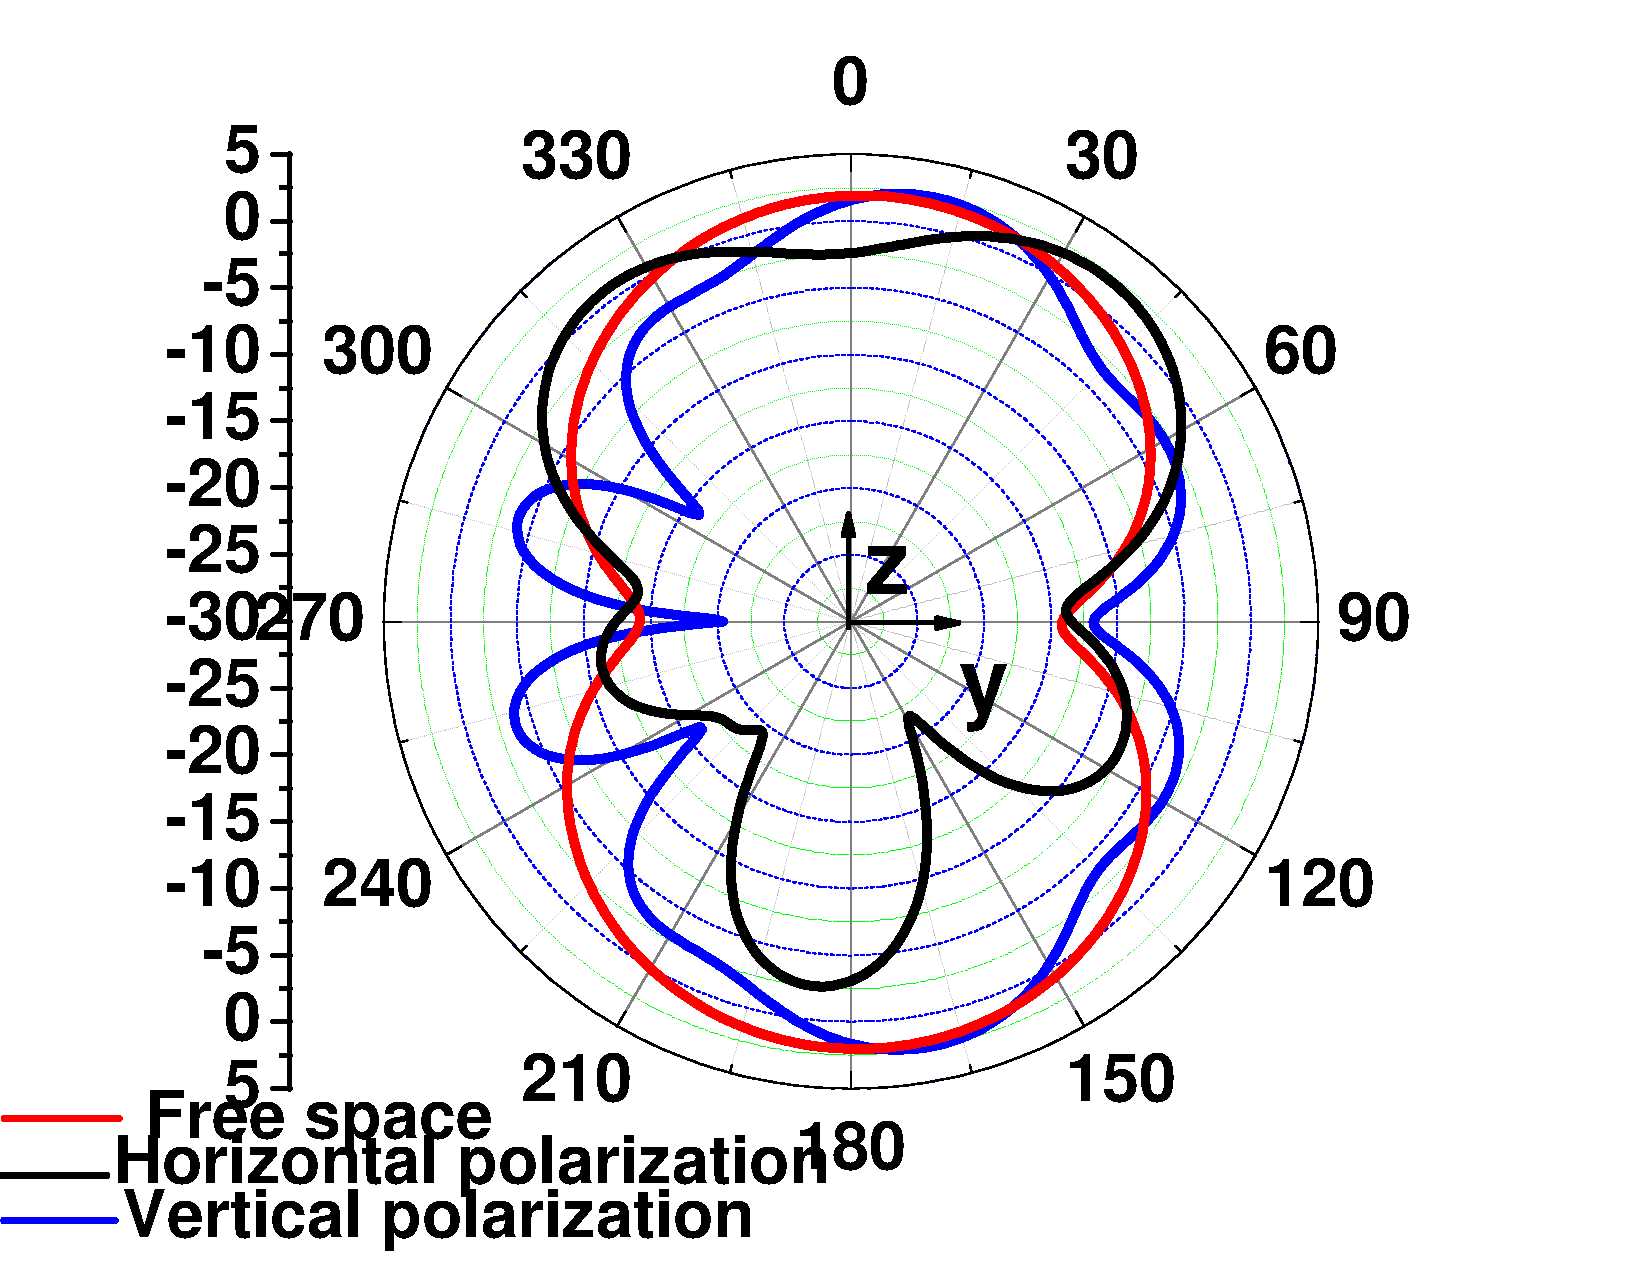
\includegraphics[width=\textwidth]{figs/10a.pdf}
\caption{E-plane}
\label{fig:10a}	
\end{subfigure}		
\begin{subfigure}[b]{0.24\textwidth}
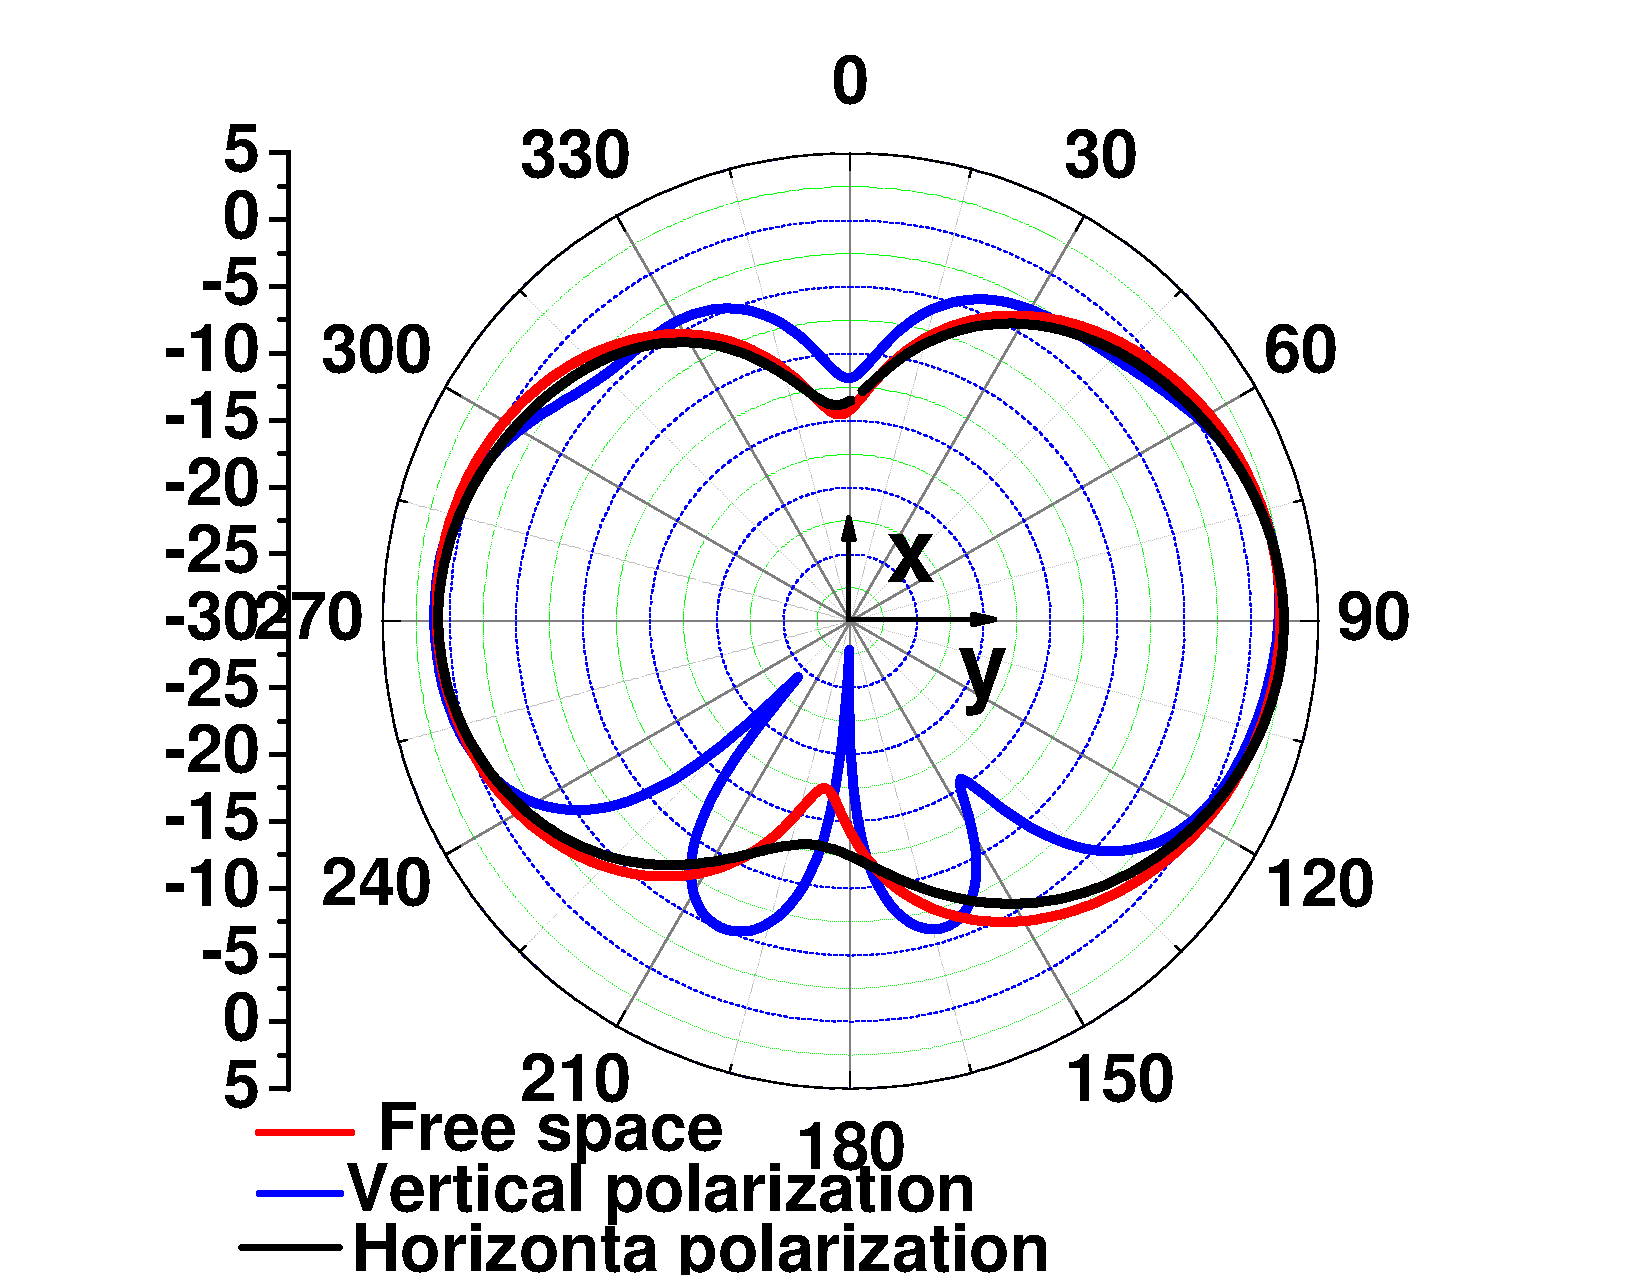
\includegraphics[width=\textwidth]{figs/10b.pdf}
\caption{H-plane}
\label{fig:10c}	
\end{subfigure}
\begin{subfigure}[b]{0.24\textwidth}
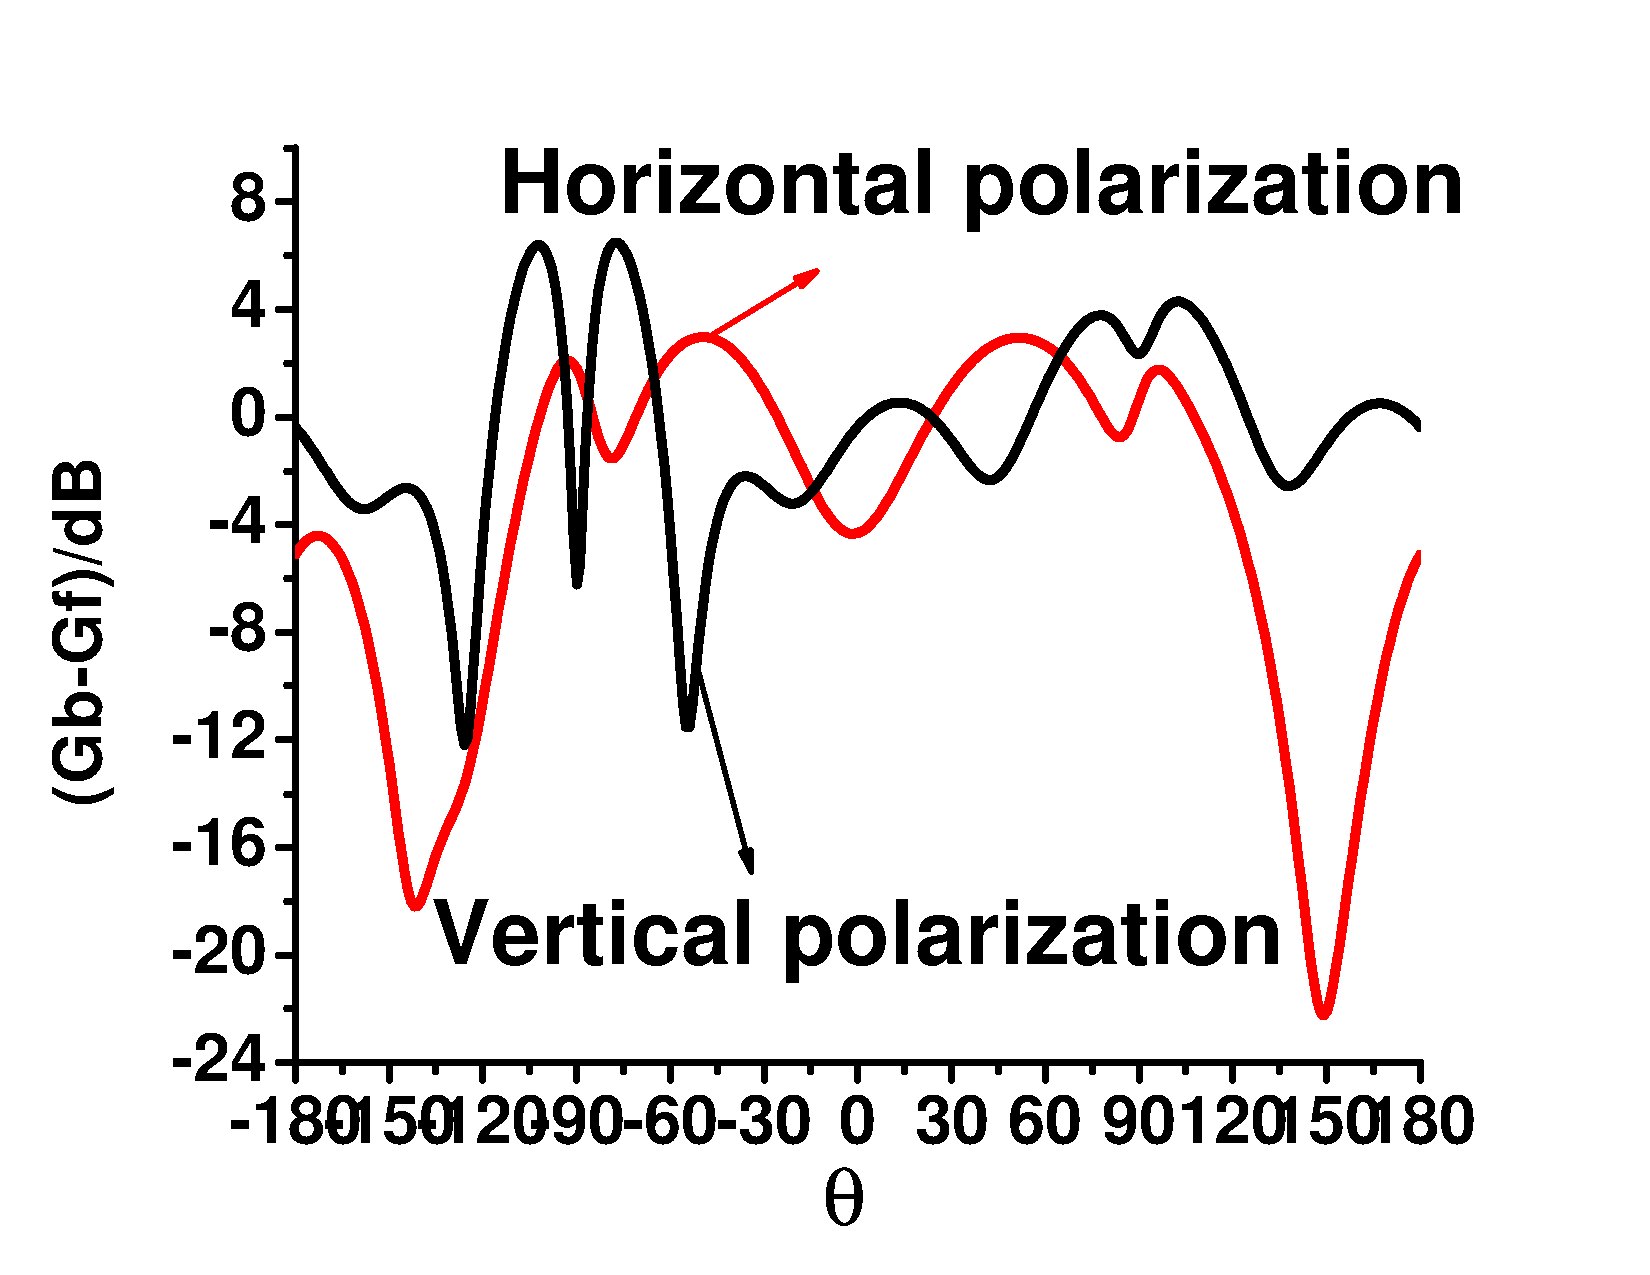
\includegraphics[width=\textwidth]{figs/10c.pdf}
\caption{Differential gain of E-plane }
\label{fig:10b}
\end{subfigure}
\begin{subfigure}[b]{0.24\textwidth}
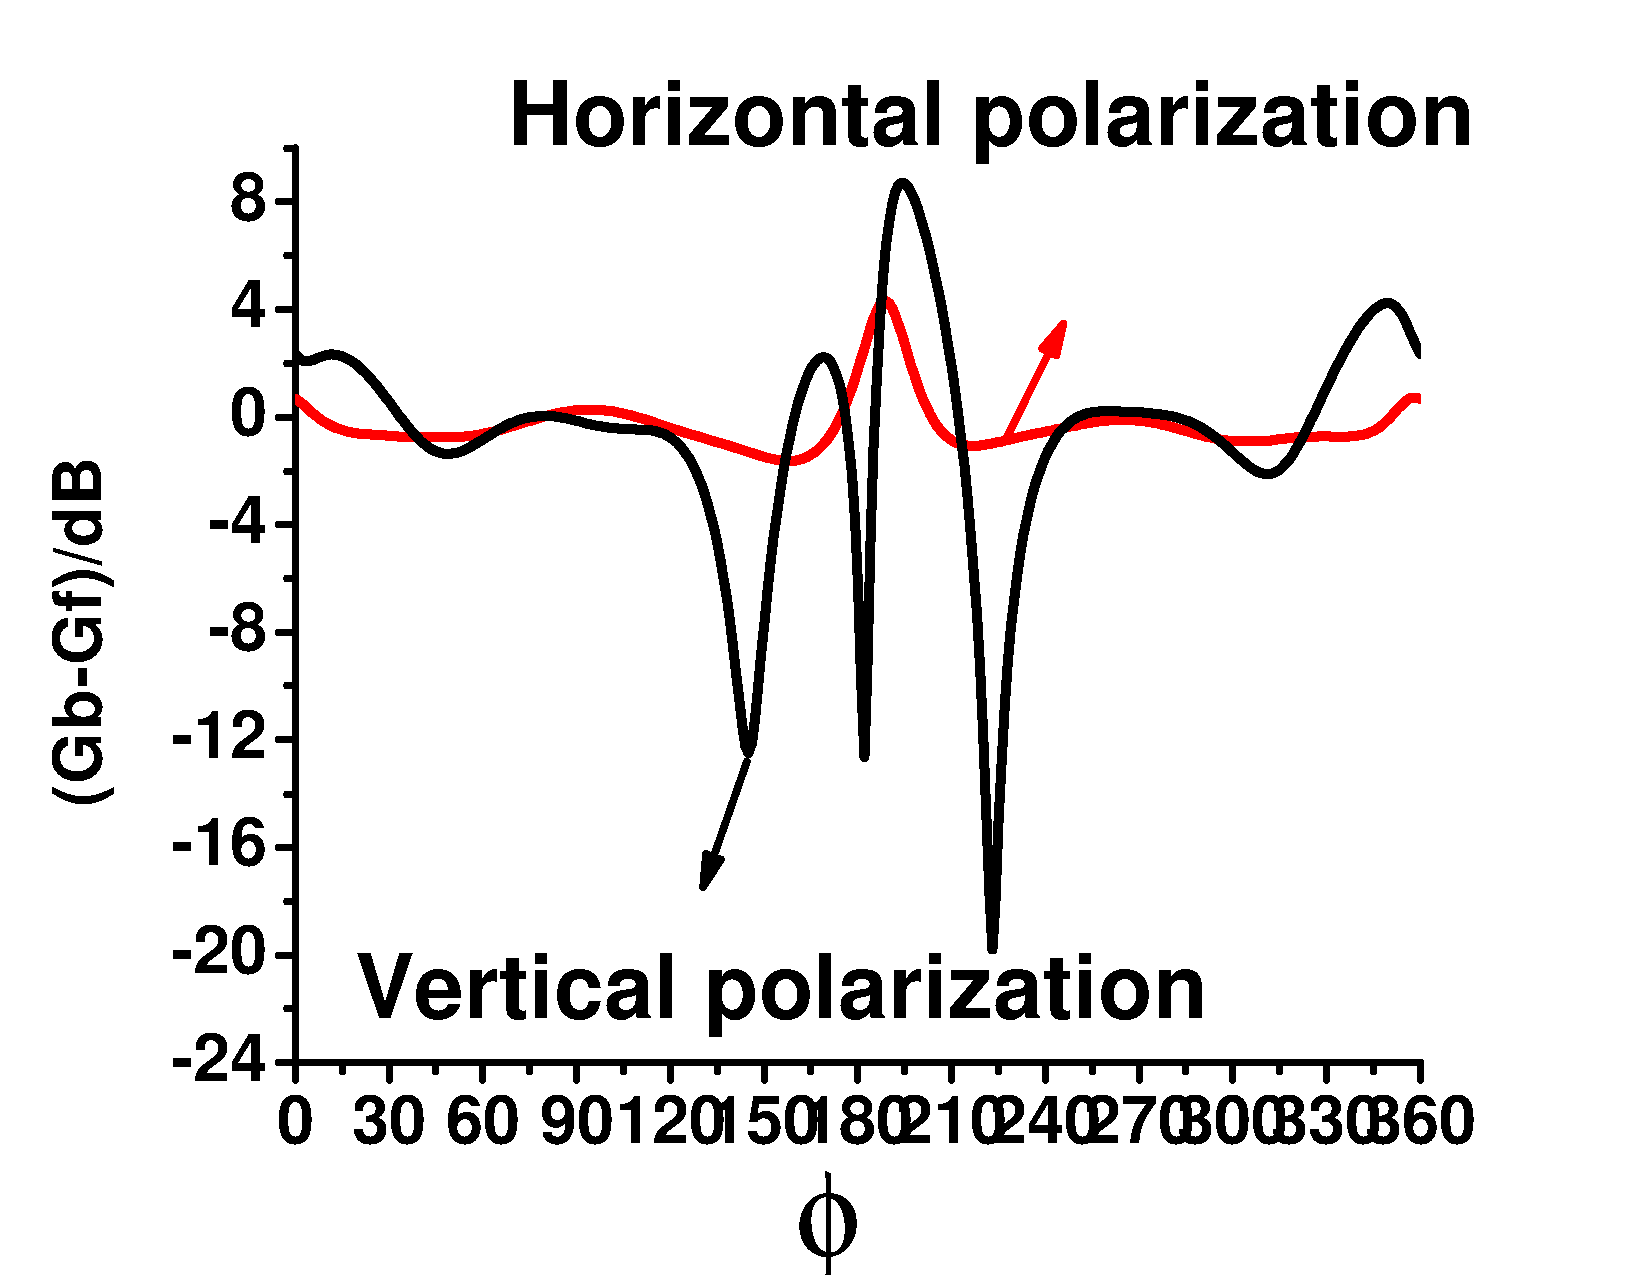
\includegraphics[width=\textwidth]{figs/10d.pdf}
\caption{Differential gain of H-plane}
\label{fig:10d}	
\end{subfigure}
\caption{Antenna gain pattern}
\label{fig:10}
\end{figure}
fig. \ref{fig:9} shows the radiation pattern of the antenna in free space and after loading body model. Horizontal
polarization and vertical polarization were selected 5.5cm and 4cm respectively as the research focus.
The gain pattern of horizontal polarization and vertical polarization after loading human body model is symmetrically
distributed with  $0\,^{\circ}$ and $90\,^{\circ}$ respectively. For horizontal polarization, the fitted curve equation of
gain difference is
\begin{equation}
\label{eq:eps_5}
y[dB]=-4.5676x^2-0.0018x+1.1592, x[cm]
\end{equation}
At the position of $-180\,^{\circ}$\textless$\theta$\textless$-110\,^{\circ}$,
$110\,^{\circ}$\textless$\theta$\textless$180\,^{\circ}$, $\mid$$G_{b}$-$G_{f}$$\mid$\textgreater4, the human body has a
significant effect on antenna gain pattern. When $\theta$=$150\,^{\circ}$, $\mid$$G_{b}$-$G_{f}$$\mid$ takes the maximum, the
human body has the greatest effect on antenna gain pattern. For vertical polarization, at the position
of$-135\,^{\circ}$\textless$\theta$\textless$120\,^{\circ}$, $-65\,^{\circ}$\textless$\theta$\textless$-45\,^{\circ}$,
$\mid$$G_{b}$-$G_{f}$$\mid$\textgreater6, the effect of the body on antenna gain pattern is obvious; when
$\theta$=$130\,^{\circ}$and $\theta$=$550\,^{\circ}$, $\mid$$G_{b}$-$G_{f}$$\mid$=12, reaches the maximum, human body has the
greatest effect on antenna gain pattern.

For H-plane gain pattern of the horizontal polarization, the gain curve is always gentle and the body has little effect on
antenna gain pattern. For vertical polarization, the curve fluctuates obviously at the position of
$145\,^{\circ}$\textless$\theta$\textless$230\,^{\circ}$, the human body has great effect on antenna.
$\mid$$G_{b}$-$G_{f}$$\mid$ takes the maximum and the human body has the most obvious effect on antenna.
subsection{Printed dipole}
\begin{figure}[!htb]
\centering
\begin{subfigure}[b]{0.4\textwidth}
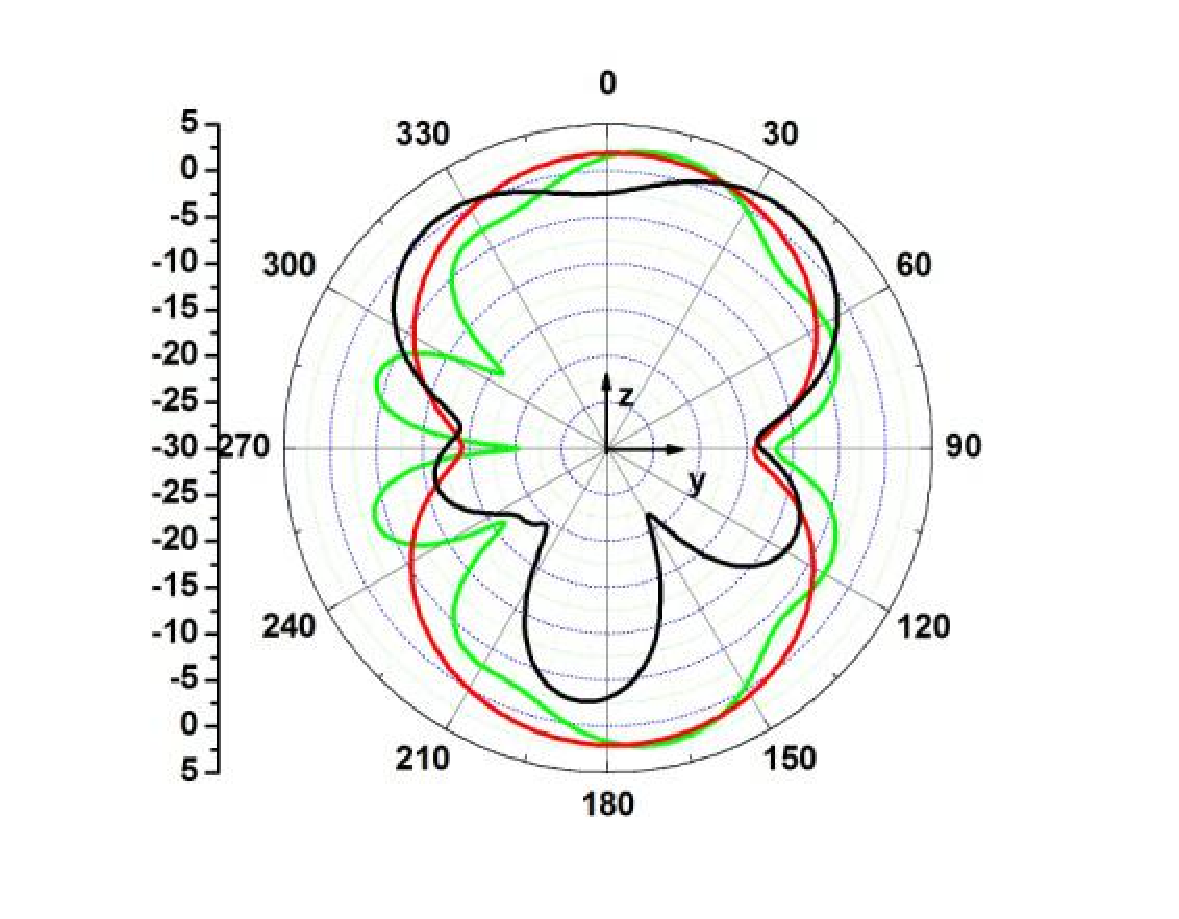
\includegraphics[width=\textwidth]{figs/11a.eps}
\caption{S11 changes}
\label{fig:11a}	
\end{subfigure}		
\begin{subfigure}[b]{0.4\textwidth}
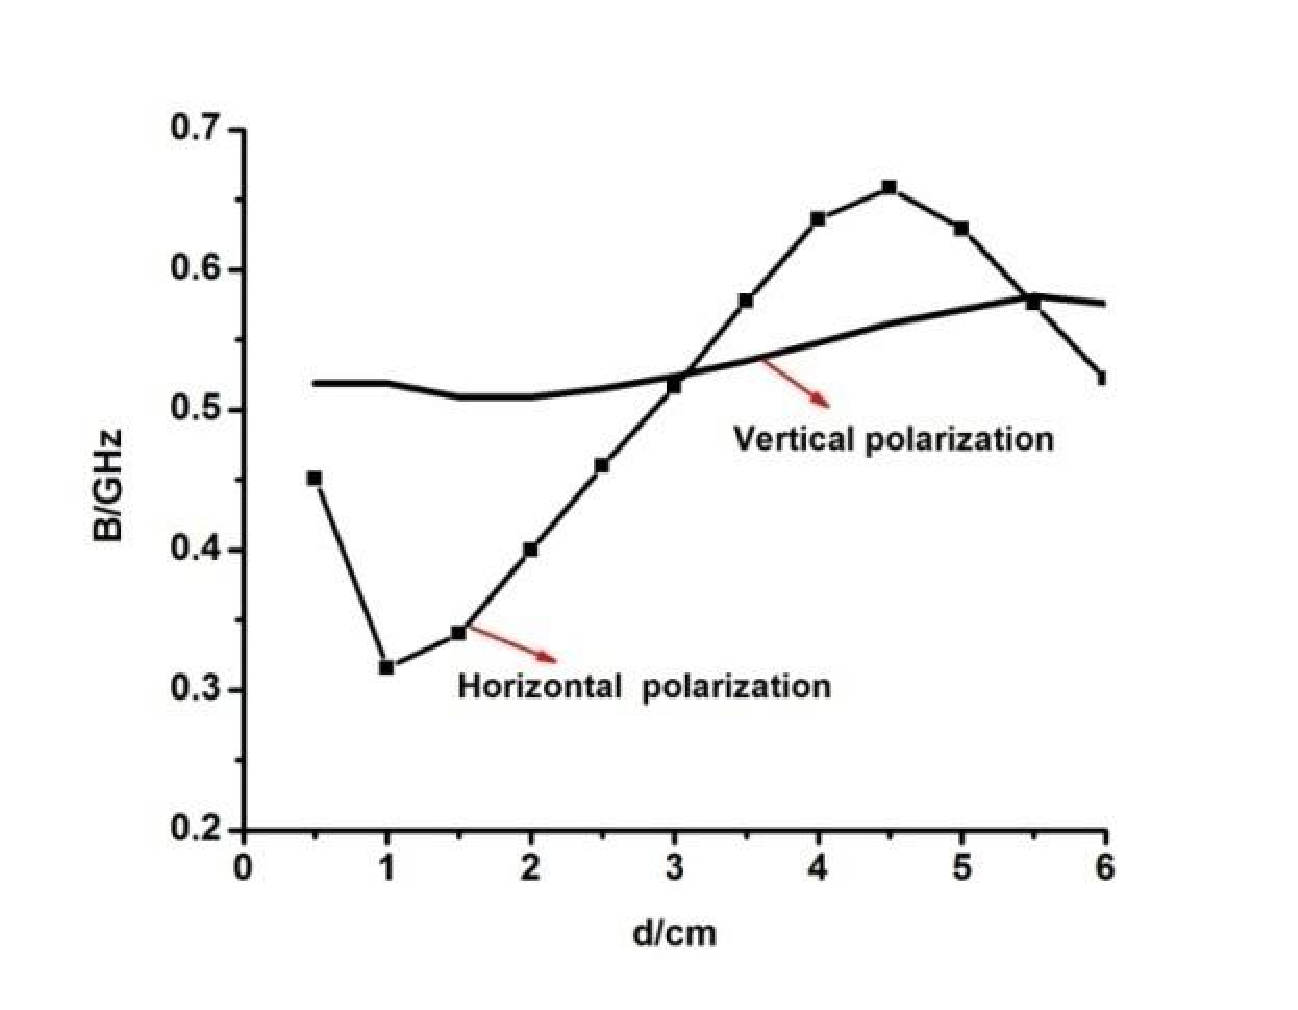
\includegraphics[width=\textwidth]{figs/11b.eps}
\caption{B changes}
\label{fig:11b}
\end{subfigure}
\caption{Comparison of S11 and B of horizontal polarization and vertical polarization with different \textit{d}}
\label{fig:11}
\end{figure}
For horizontal polarization, the fitting curve equation of bandwidth is
\begin{equation}
\label{eq:eps_6}
y[dB]=0.014x+0.4937, x[cm]
\end{equation}
When \textit{d}=1cm, the bandwidth is narrowest, the antenna is not suitable for placing on body surface at this time. For
vertical polarization, the fitted curve equation of bandwidth is
\begin{equation}
\label{eq:eps_7}
y[dB]=-0.0153x^2-0.2802x+0.52222, x[cm]
\end{equation}
At the range of all distances, when \textit{d}=3cm, S11 takes the minimum, so when the antenna placed 3cm near the body
surface in vertical polarization, the antenna performance is the best. We can see form the S11 curve, the trend of vertical
polarization and horizontal polarization is consistent, and the fitting curve equation is
\begin{equation}
\label{eq:eps_8}
y[dB]=-0.838x-37.197, x[cm]
\end{equation}
\begin{equation}
\label{eq:eps_9}
y[dB]=-3.4777X-12.723, x[cm]
\end{equation}
\begin{figure}[!htb]
\centering
\begin{subfigure}[b]{0.24\textwidth}
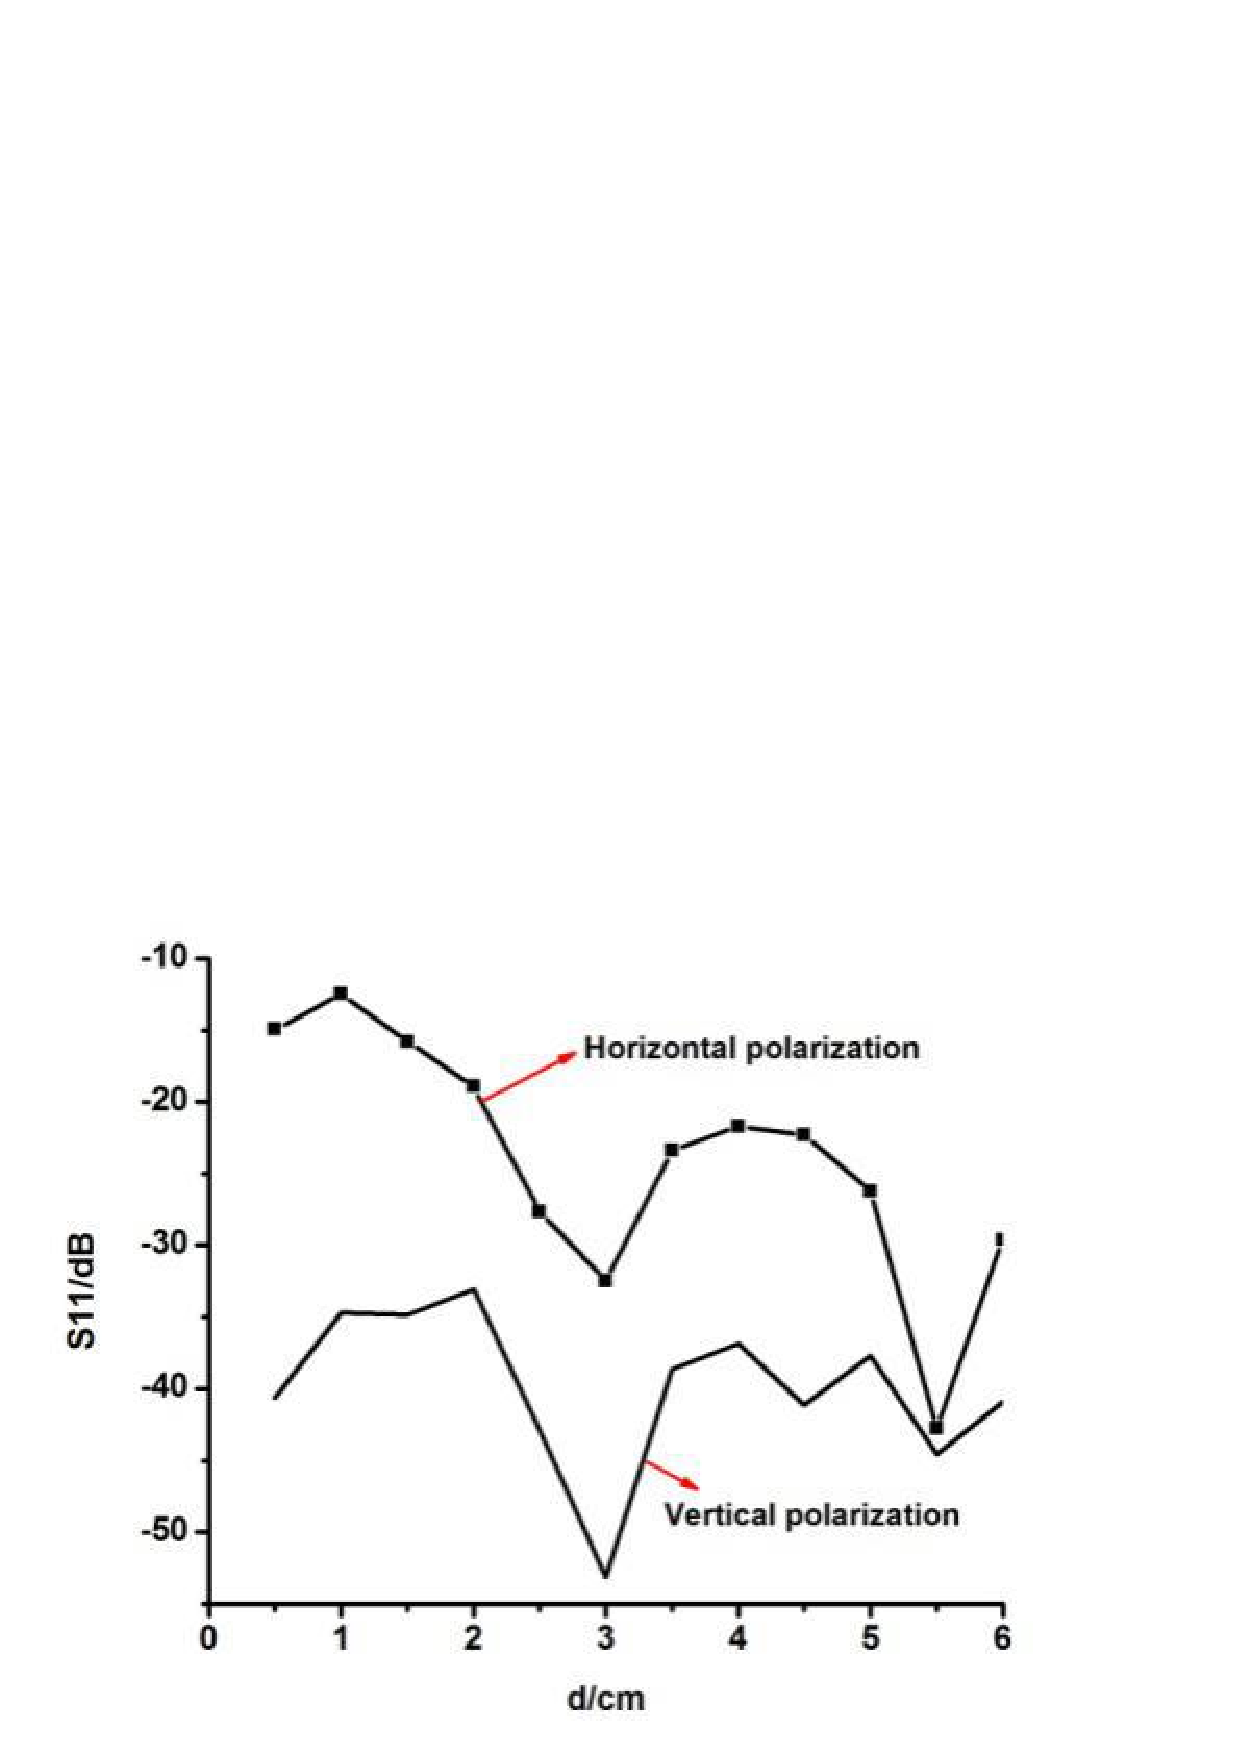
\includegraphics[width=\textwidth]{figs/12a.pdf}
\caption{Horizontal polarization of E-plane}
\label{fig:12a}	
\end{subfigure}		
\begin{subfigure}[b]{0.24\textwidth}
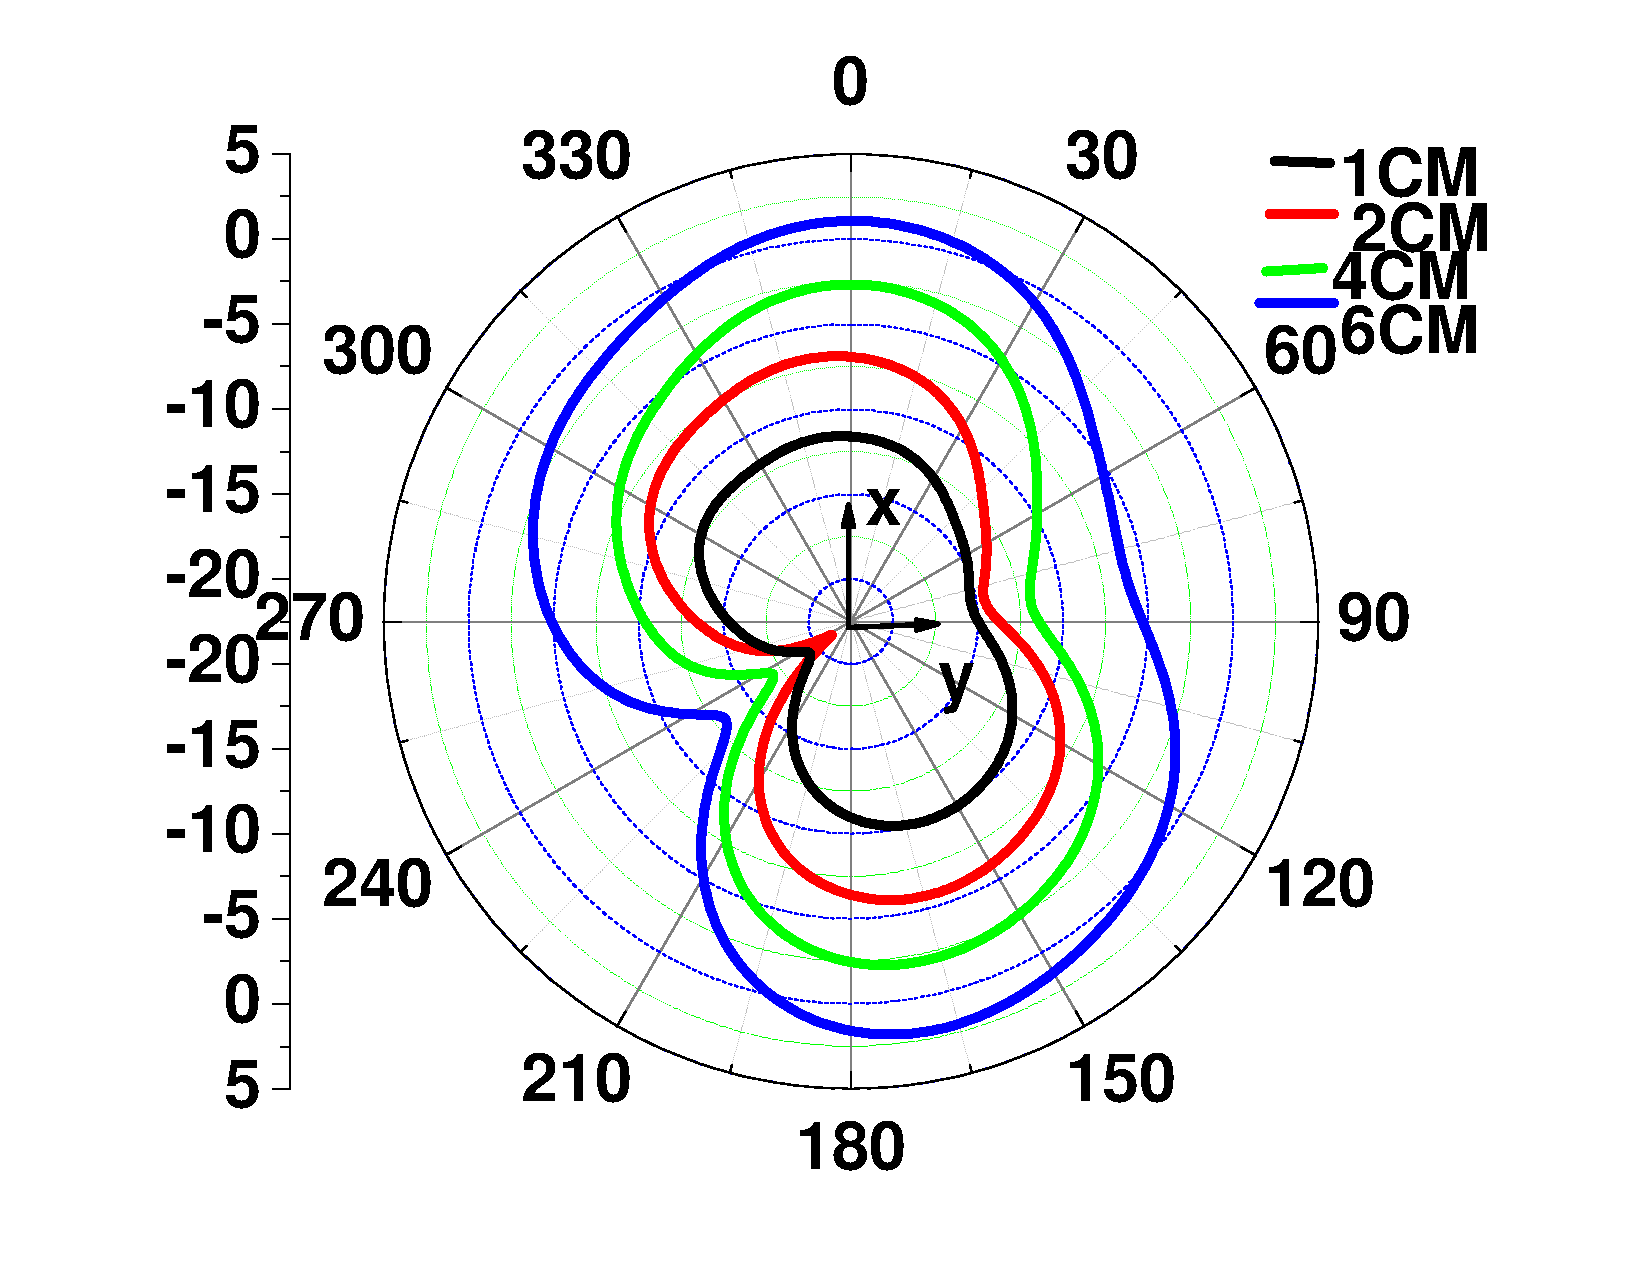
\includegraphics[width=\textwidth]{figs/12b.pdf}
\caption{Horizontal polarization H-plane}
\label{fig:12b}	
\end{subfigure}
\begin{subfigure}[b]{0.24\textwidth}
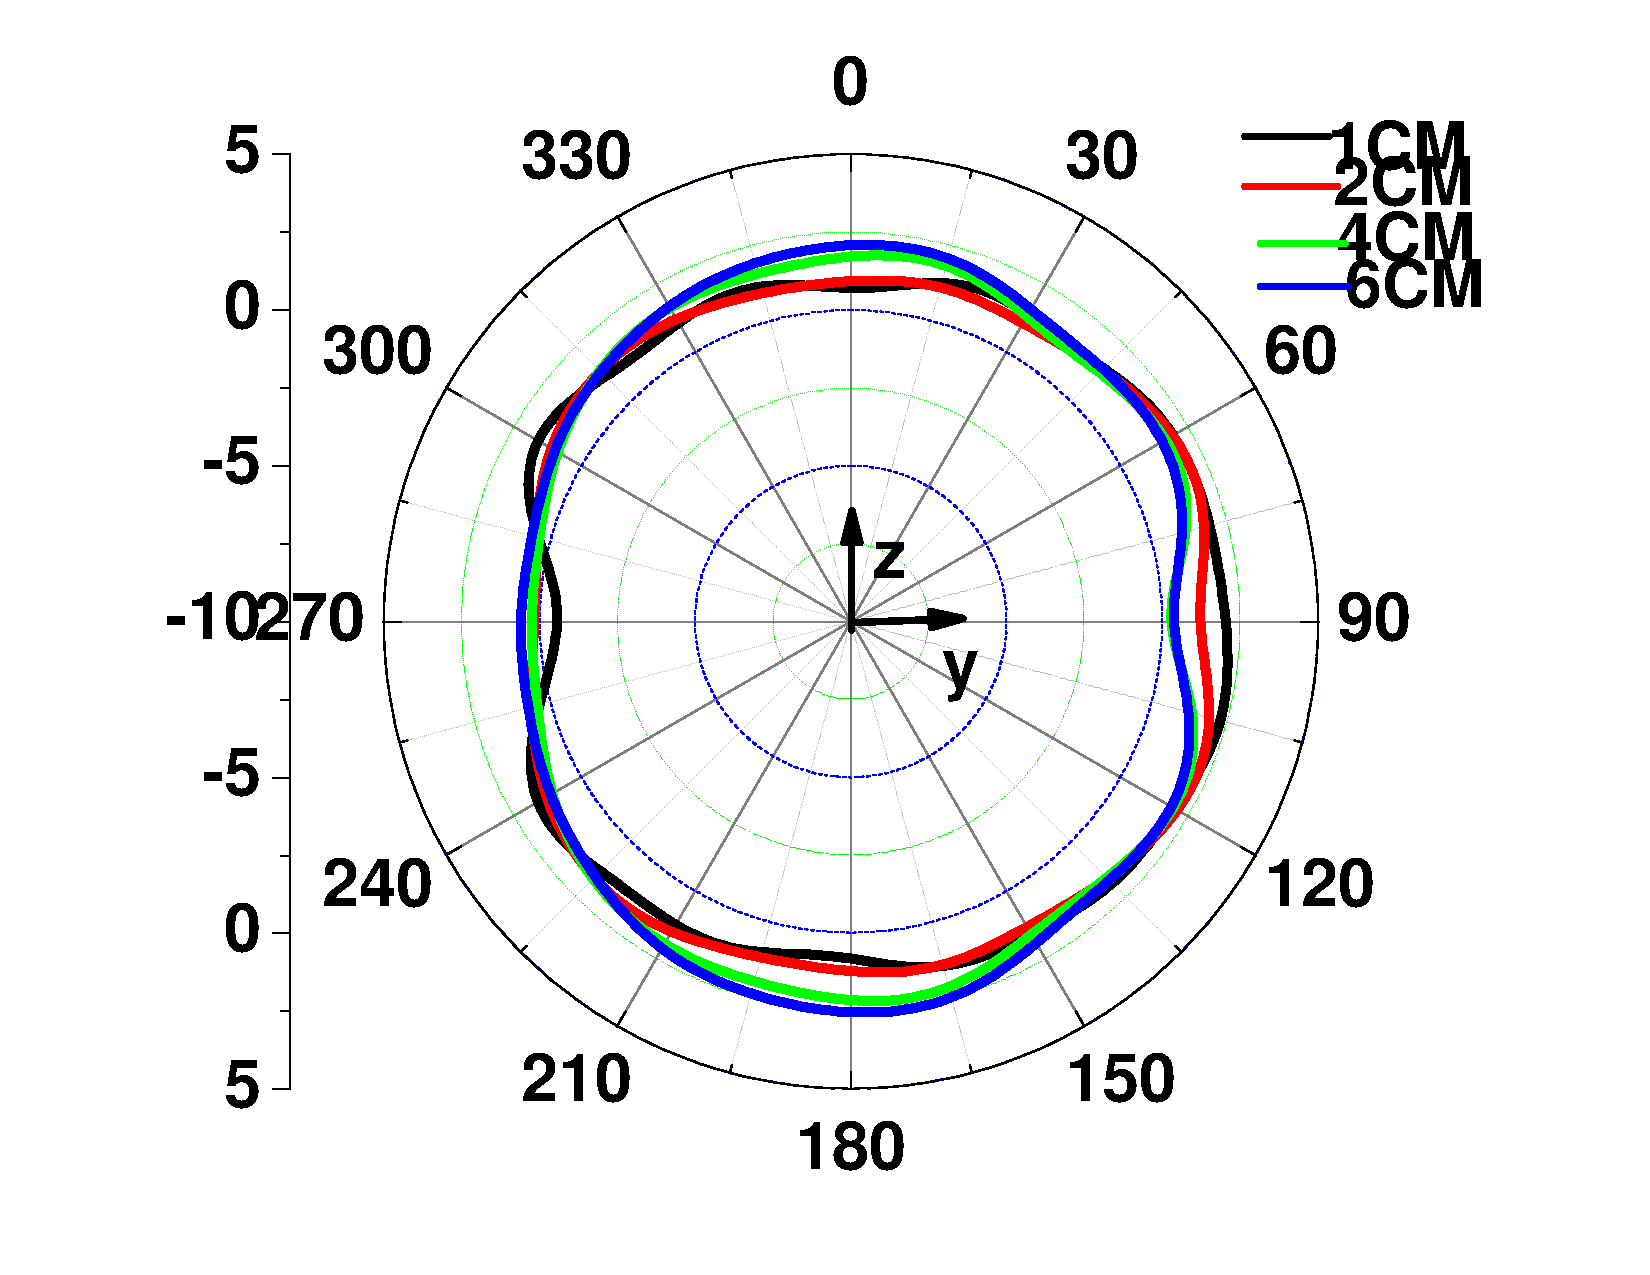
\includegraphics[width=\textwidth]{figs/12c.pdf}
\caption{Vertical polarization E-plane}
\label{fig:12c}
\end{subfigure}
\begin{subfigure}[b]{0.24\textwidth}
\includegraphics[width=\textwidth]{figs/12d.pdf}
\caption{Vertical polarization of H-plane}
\label{fig:12d}	
\end{subfigure}
\begin{subfigure}[b]{0.24\textwidth}
\includegraphics[width=\textwidth]{figs/12e.pdf}
\caption{E-plane}
\label{fig:12e}	
\end{subfigure}
\begin{subfigure}[b]{0.24\textwidth}
\includegraphics[width=\textwidth]{figs/12f.pdf}
\caption{H-plane}
\label{fig:12f}	
\end{subfigure}
\caption{Comparison of gain pattern of horizontal polarization and vertical polarization of \textit{d}}
\label{fig:12}
\end{figure}
Horizontal polarization and vertical polarization take the minimum and maximum at \textit{d}=3cm and \textit{d}=5.5cm respectively. S11 of horizontal polarization is always greater than vertical polarization. When 0cm$<\textit{d}<$3cm, the bandwidth of vertical polarization is always greater than horizontal Polarization. Therefore, in this range of \textit{d}, the antenna is more suitable for vertical polarization.
For horizontal polarization, as shown in fig. \ref{fig:12a} and fig. \ref{fig:12d}, the directional gain distributions at different distances are relatively uniform and are not sensitive to d; but within the range of \textit{$\theta$} and \textit{$\varphi$}, 2\textless$S^{2}$\textless7, $S^{2}$ is large and the difference in gain is relatively large at different distances in the same direction.

For vertical polarization, as shown in fig. \ref{fig:12b} and fig. \ref{fig:12e}, the E-plane pattern is stable and is not sensitive to \textit{d}. At the position of $85\,^{\circ}$\textless$\varphi$\textless$90\,^{\circ}$, $120\,^{\circ}$\textless$\varphi$\textless$130\,^{\circ}$, $220\,^{\circ}$\textless$\varphi$\textless$230\,^{\circ}$, $S^{2}$\textgreater7, the difference of H-plane pattern of \textit{d} is relatively great, the antenna direction gain is more sensitive to \textit{d}.

\ifCLASSOPTIONcaptionsoff
  \newpage
\fi



\begin{thebibliography}{1}
\bibitem{1}
 Hall P S, Hao Y. Antennas and propagation for body centric communications. Norwood, MA: Artech House, 2006.

\bibitem{2}
 Hall P S,  ��Antennas and propagation for body centric wireless communications,�� in Proc. IET Seminar on antennas and Propagation for Body-Centric Wireless Communications, pp. 1-4, 2007.

 \bibitem{3}
 Hall P S. ��Diversity in on-body communications channels�� in Proc. 2008 International Workshop on Antenna Technology, Chiba, Japan, pp. 5-9, 2008.

 \bibitem{4}
 Conway G A, Scanlon W G, Cotton S L. The performance of on-body wearable antennas in a repeatable multipath environment[C]//Antennas and Propagation Society International Symposium, 2008. AP-S 2008. IEEE. IEEE, 2008: 1-4.

\bibitem{5}
Salonen P, Rahmat-Samii Y, Kivikoski M. Wearable antennas in the vicinity of human body[C]//Antennas and Propagation Society International Symposium, 2004. IEEE. IEEE, 2004, 1: 467-470.

\bibitem{6}
Jensen M A, Rahmat-Samii Y. EM  interaction of handset antennas and a human in personal communications[J]. \emph{Proceedings of the IEEE},1995,83(1):1-17
\bibitem{7}

Iskander, M. E., Zhengqing Yun, and R.Quintero-Illera.``Polarization and human body effects on the microwave absorption in a human head exposed to radiation from handheld devices.''
\emph{IEEE Transactions on Microwave Theory and Techniques}, 2000, 48(11): 1979-1987.

\bibitem{8}
Hurme H, Salonen P, Rantanen J, et al. On the Study of Antenna Placement in a Smart Clothing[C]//\emph{Modelling and Simulation}, 2003: 1-6.

\bibitem{9}
Nechayev Y I, Constantinou C C, Wu X, et al. De-polarization of on-body channels and polarization diversity at 60 GHz[J]. IEEE Transactions on Antennas and Propagation, 2014, 62(12): 6519-6523.
\bibitem{10}
Shimizu Y, Furukawa T, Anzai D, et al. Performance improvement by transmit diversity technique for implant ultra-wideband communication[J]. IET Microwaves, Antennas
\& Propagation, 2016, 10(10): 1106-1112.

\bibitem{11}
Wei W Y, Gong D M, Chen B S. Antenna theory[M].Xi��an: Publishing House of School of Electronic Engineering, Xidian University, 1994

\bibitem{12}
Klemm M, Troester G. Textile UWB antennas for wireless body area networks[J]. \emph{Transactions on Antennas and Propagation}, 2006, 54(11): 3192-3197.

\bibitem{13}
Wang Z, Zhang L, Psychoudakis D, et al. Flexible textile antennas for body-worn communication[C]//Antenna Technology (iWAT), \emph{2012 IEEE International Workshop on. IEEE}, 2012: 205-208.

\bibitem{14}
Wang Z, Zhang L, Bayram Y, et al.Embroidered conductive fibers on polymer composite for conformal antennas[J]. \emph{IEEE Transactions on Antennas and Propagation}, 2012, 60(9): 4141-4147.

\bibitem{15}
LI M Y, LIU M, Yang F.HFSS Antennas DESGIN[M]. Beijing: Publishing House of Electronic Industry, 2011:196-218, 51-53.

\bibitem{16}
Andersen A. Small size 2.4 GHz PCB antenna[J]. Texas Instruments, Application Note AN043, 2008.

\bibitem{17}
Psychoudakis D, Volakis J L. Conformal asymmetric meandered flare (AMF) antenna for body-worn applications[J].
\emph{IEEE Antennas and Wireless Propagation Letters}, 2009, 8: 931-934.

\bibitem{18}
Dimbylow P J, Gandhi O P. Finite-difference time-domain calculations of SAR in a realistic heterogeneous model of the head for plane-wave exposure from 600 MHz to 3 GHz[J]. \emph{Physics in Medicine and Biology}, 1991, 36(8): 1075.
\end{thebibliography}

\end{document}

